\documentclass[a4paper]{report}
\usepackage[T1]{fontenc}
\usepackage[utf8]{inputenc}
\usepackage[english]{babel}
\usepackage{titlesec}
\usepackage{lipsum}
\usepackage{booktabs}
\usepackage{hyperref}
\usepackage{graphicx}
\usepackage{float}
\usepackage{rotating}
\usepackage[dvipsnames]{xcolor}
\usepackage{listings}
\usepackage{alloy-style}
\usepackage[shortlabels]{enumitem}
\usepackage{geometry}
\usepackage{pdflscape}
\usepackage{caption}
\usepackage{soul}
\graphicspath{{./img/}}

\begin{document}

%%The two following lines remove the line "Chapter n" at the beginning of each chapter, before the title
%\titleformat{\chapter}[display]
%  {\normalfont\bfseries}{}{0pt}{\Large}
\titleformat{\chapter}[hang] 
{\normalfont\huge\bfseries}{\thechapter}{1em}{} 

\title{eMall RASD}
\author{Enrico Brunetti, Matteo Gionfriddo}
\date{date} %%TODO

\begin{titlepage}
\begin{figure}[t]
\centering

\includegraphics[width=0.3\textwidth]{Logo}
\end{figure}
\begin{center}
    \textsc{ \LARGE{Politecnico di Milano \\}}
	\textsc{ \Large {School of Industrial and Information Engineering\\ }}
	\vspace{3mm}
	\textnormal{ \Large{Software Engineering 2 Project\\}}
	\vspace{30mm}
	\fontsize{10mm}{7mm}\selectfont 
    \textup{e-Mobility for All.}\\
    \textnormal{ \LARGE{Requirement Analysis and Specification Document\\}}
\end{center}

\vspace{18mm}

\begin{center}
    \textnormal{\large{\bf Authors:\\}}
	{\large Enrico Brunetti \\ Matteo Gionfriddo }
	\fontsize{10mm}{5mm}\selectfont 
\end{center}
\vspace{15mm}

\centering{\large{
Academic Year 2022/2023 \\
\vspace{10mm}
Milano, 21/12/2022 \\
\vspace{2mm}
Version 1.0
}}

\end{titlepage}

\newgeometry{top=3cm}
\tableofcontents
\listoffigures
\begingroup
\let\clearpage\relax %avoid to put it on a new page
\listoftables
\endgroup
\restoregeometry
\chapter{Introduction}
\section{Scope}
eMall is a system meant to provide services for charging electric vehicles and managing charging stations. This is meant both for normal people (i.e. end users) and for CPO workers.
The application domain concerns different types of world phenomena, shared phenomena and machine phenomena. \\
We can identify the followings world phenomena:
\begin{itemize}
\item {[W1]} \label{W1}User connects his electric vehicle to the charge socket.
\item {[W2]} \label{W2}DSOs provide energy to their associated charging stations.
\item {[W3]} \label{W3}Batteries, if available and enabled, store energy from DSOs and provide it to the charging station.
\item {[W4]} \label{W4}Charging sockets are supplied directly by DSO through the network and/or by batteries of the charging station.
\end{itemize}
the following shared phenomena controlled by the world and observed by the machine:
\begin{itemize}
\item {[S1]} A user books a charge in a charging station.
\item {[S2]} A user enables a charging column.
\item {[S3]} CPOs decides to take energy from DSOs and/or from batteries, if available.
\end{itemize}
and the following shared phenomena controlled by the machine and observed by the world:
\begin{itemize}
\item {[S4]} Location, external and internal status of the charging station are visible.
\item {[S5]} The system checks the booking ID and enables the charging operation.
\item {[S6]} Vehicle charging is started.
\item {[S7]} Vehicle charging is stopped and a notification is sent.
\item {[S8]} The system elaborates the payment of the charging service.
\end{itemize}

\section{Purpose}
The system is characterized by the following goals:
\begin{itemize}
\item{[G1]} \label{G1}Users must know position, prices and special offers of charging stations.
\item {[G2]} \label{G2}Users must be able to complete the whole process of charging for their electric vehicles.
\item  {[G3]} \label{G3}CPOs workers must be able to manage charging stations associated to their CPO.
\item  {[G4]} \label{G4}CPOs must be able to communicate with DSOs in order to provide energy furniture.
\end{itemize}

In the following table is shown which world and shared phenoma are involved for each goal.
\begin{table}[H]
  \centering
  \begin{tabular}{|c|c|c|c|c|c|c|c|c|c|c|c|c|}
    \cline{2-13}
    \multicolumn{1}{c|}{} & W1 & W2 & W3 & W4 & S1 & S2 & S3 & S4 & S5 & S6 & S7 & S8\\ \hline
    G1 &   &   &   &   & X &   &   & X &   &   &   &   \\ \hline
    G2 & X & X & X & X & X & X &   &   & X & X & X & X \\ \hline
    G3 &   & X & X & X &   &   & X & X &   &   &   &   \\ \hline
    G4 &   & X &   &   &   &   & X &   &   &   &   &   \\ \hline
  \end{tabular}
  \caption{Correspondence between goals and world and shared phenoma}
\end{table}


\section{Definitions, acronyms and abbreviations}
\begin{itemize}
\item \textit{eMSP}: e-Mobility Service Provider.
\item \textit{CPO}: Charging Point Operator.
\item \textit{CPOW}: Charging Point Operator Worker.
\item \textit{CPMS}: Charge Point Management System.
\item \textit{DSO}: Distribution System Operator.
\end{itemize}
\section{Revision history}
\begin{itemize}
\item 21/12/2022 Version 1.0.
\end{itemize}
\section{Reference documents}
\begin{itemize}
\item Assignment Document "Assignment RDD AY 2022-2023\_v3.pdf".
\end{itemize}
\section{Document structure}

The document consists of 6 different chapters:
\\
\\
\textbf{Chapter 1}: in this first chapter the application domain is presented starting with the scope, which includes world and shared phenomena that the application can observe and/or control. Furthermore, in the purpose section, the main goals are presented and at the end, some basic information is provided in order to help in the understanding of the whole document.\\ \\
\textbf{Chapter 2}: the second chapter starts with an overall description of the whole application, made by the definition of the most important possible scenarios which will involve the different types of users and their relationships with the eMall system. Some UML diagrams, i.e. class diagram and state diagrams, are here provided to help to understand which are the different entities of the system and how they should work together in order to provide all required functionalities. The chapter contains also an exhaustive explanation of the main product functions, a description of the different actors, and a list of all needed domain assumptions.\\ \\
\textbf{Chapter 3}: the third chapter is the heart of the RASD document. First of all external interface and functional requirements are defined and then the second ones are mapped into goals that satisfy and domain assumptions that exploit. Subsequently, the behavior of the system is described by use cases, which are enriched with use cases and sequence UML diagrams. The chapter then ends with performance requirements, design constraints, and software system attributes.\\ \\
\textbf{Chapter 4}: the fourth is the last effective chapter of the RASD document. It contains a formal analysis of the problem presented using the alloy modeling language. It is especially used to formally verify the consistency of functional requirements.\\ \\
\textbf{Chapter 5}: in this chapter, the effort spent by each team member is briefly presented in order to provide an overview of how the work has been done.\\ \\
\textbf{Chapter 6}: the last chapter contains the references used during the developing process of the document.

\chapter{Overall Description}
\section{Product perspective}
This section is dedicated to the identification of the most important scenarios and to a first description of the whole system through class and state diagrams.
\subsection{Scenarios}
For all scenarios described below we assume that the system provides a mobile application for end users and a web interface for CPOWs.
\subsubsection{Unregistered end-user}
A possible end-user has just bought his brand new Tesla Model X and has seen some interesting ads from a famous eMSP about the new application eMall, which will allow him to know where to charge his vehicle and manage the whole process. He decides to download the app and sign-up, filling in all the requested fields and starting using the app. He decides also to insert a picture of his driving license and to register his car inserting dates about the model and the plate. After that, he will include also all information about his debit card so, when he will decide to book a recharge everything will be ready.

\subsubsection{Unregistered CPOW}
A new CPOW has just been hired and on his first day of work, he needs to register to the eMall web service in order to manage the CPMS of the CPO he is working for. During the sign-up process, he has to insert, in addition to all requested fields, also a special code provided by his employer to register him as a CPOW of that particular CPO.

\subsubsection{End-user wants to book a charge}
An end-user decides to open eMall app in order to see if there are new offers in the charging stations of his city and discovers that the one of the shopping mall has a discount of 25\%. Tomorrow he will finish working at 6:30 pm and he needs to buy also a pair of shoes. So he decides to take advantage also of the special offer and clicks on the book button of the charging station on the map, selects his car and a payment method, and books a fast charging socket between 7 pm and 8 pm tomorrow.

\subsubsection{End-user charges his vehicle}
An end user arrives at the charging station where he has booked a medium-speed charging socket, presses the unlock button from the app, connects the socket to his car, and starts the charging process. Now he goes to get his hair cut and while he was looking at his new hairstyle in front of the mirror he receives a notification from eMall app which says that the charging process is finished. So he comes back to the charging station, presses the disconnect button on the app, and disconnects the charging socket. At this point, he receives a notification from his bank which says that 20 euros have been charged to his debit card.

\subsubsection{CPOW registers a newly opened charging station}
A CPOW has just received the assignment to manage through the CPMS a new charging station that will be inaugurated today in the main square of the city, that can be accessed only by electric vehicles. Since all connections between the station and the systems have been already configured by technicians he only has to add it on his web interface. He presses the \textit{configure new station} button and fills all requested fields taking special care about the unique physical id identifier of the station that will allow him to manage it from his CPMS. At this point, the charging station configuration is ended and the management can start to work properly.

\subsubsection{CPOW temporarily disable batteries due to maintenance}
This night 4 batteries of charging station 1046 have to be removed following the regular maintenance schedule and a CPOW that manages the CPMS related to that charging station has to do some operations before the end of his turn at 6 pm. First of all, he selects that specific charging station on his web interface clicks the battery management button, and selects the 4 interested batteries. At this point, he selects programmed disabling and sets the batteries off from 9 pm of that evening. Since the recharging station has 2 more batteries he sets up to take 25\% of energy from batteries and 75\% directly from DSO during the charging processes of that night. The day after when the CPOW starts his turn at 9 am he receives a notification that the maintenance has ended and batteries have been correctly reconnected. So he re-enables them and set the charging station to take again 100\% of energy from batteries.

\subsubsection{CPOW shows to his manager dates about a charging station}
Yesterday a new charging station has been opened in the parking of the city shopping center and this morning the manager knocks on the door of the office of the CPOW who manage, trough the CMPS, that specific station, in order to see if there are already some users. The CPOW opens his web interface, selects charging station 1050, and clicks on show statistics. The charging station is composed of 6 charging sockets, 3 at fast-speed and 3 at medium-speed, and 10 batteries. Currently, 2 cars are charging: the first one is a Honda-e, connected to socket 1 (fast-speed charge), that has absorbed 19/35.5kwh of power and will take 12 minutes to complete the charging process. The second one is a Hyundai	Kona Electric, which is connected to socket 4 (medium-speed charge), that has absorbed 10/64kwh of power and will take 55 minutes to complete the charging process. The CPOW and the manager see also that 12 other recharges have been booked from now to midnight, 7 on fast-speed sockets and 5 on medium-speed ones. Actually only one of the 10 batteries is at 53\% of his charge and the remaining 9 are all full. The manager is pretty satisfied since it is only the second day since the station has opened and he can see encouraging results. So he invites the CPOW for a coffee break and they go to the coffee machine together.

\subsubsection{CPOW manually decides where to get energy}
A CPO company made a deal with a DSO company and if they will purchase energy only from them for one month they will reduce the price making it the most convenient for the CPO. So all CPOWs of the interested CPO have been instructed to proceed in this way. We took as an example one of them. This specific CPOW decides to have a look at the different offers from all available DSO and he notices that actually the one of the deal isn't the cheaper, so the system won't dynamically decide to acquire energy from that specific company. So, through the web interface of the CMPS, he switches off the auto-deciding acquisition for all the charging stations under his control and set the specific DSO as the only supplier. He also sets all charging stations to use only energy from the batteries until they are empty trying to save some money using before all the already purchased energy that is available.

\subsection{Class diagram}
The UML class diagram which describes the domain application is presented in figure \ref{fig:class-diagramRASD}. The User class is abstract and both EndUser and CPOW classes inherit from it since are the two different types of users of the whole system. Each EndUser is registered to at least one eMSP, owns vehicles and can book recharges which refer to them. Each recharge has a status and happens in a charging socket of a charging station related to one of the eMSP that the user is registered to. Charging stations are composed of charging columns which are in turn composed of charging sockets and optionally also of batteries. There can be discounts associated to them. Each charging station refers to a specific eMSP. Each CPO administrates one and only one CPMS that manages one or more charging stations and can use DSOs to purchase energy forniture. There is a provisional class that is EnergyForniture, because at this stage of the project the best way to keep track of energy furniture is to separate them and locate different bills in different objects. This is meant in order to have a detailed report of the precise amount of energy purchased, its price and its destination since each energy forniture can refer to one/more batteries or directly to one/more charging sockets.

\subsection{State charts}
\subsubsection{Charging process}
In the state chart displayed in figure \ref{fig:state-diagramRASD} the whole charging process is presented. This chart starts describing the booking process and all the requirements that have to be satisfied in order to make a correct booking of a charge (i.e. vehicle selection).  For simplicity, we assume that the user is already logged in to the application and that the \textit{select charging station} operation is meant to include also the type of socket if more options are available (i.e. fast charge socket). After the charge is booked, when the user inserts the plug of his vehicle into the socket the system enters the \textit{Waiting charge completed} state, which is composed of two different states that describe the effective charging process. When the plug is removed the whole process ends. With this last action, we assume also that the payment is done at the moment of the plug removal since the found availability has been already checked during the booking phase.

\subsubsection{Charging station energy supply}
In the state chart displayed in figure \ref{fig:state-diagramChargingRASD} is described the state machine related to the energy supply types of a charging station. This representation has to be assumed to be applied independently to all the charging sockets of that specific charging station and the selection between batteries and network can be made manually by CPMS operators or dynamically by the system.

\newgeometry{top=0.1cm}
\begin{figure}[p]
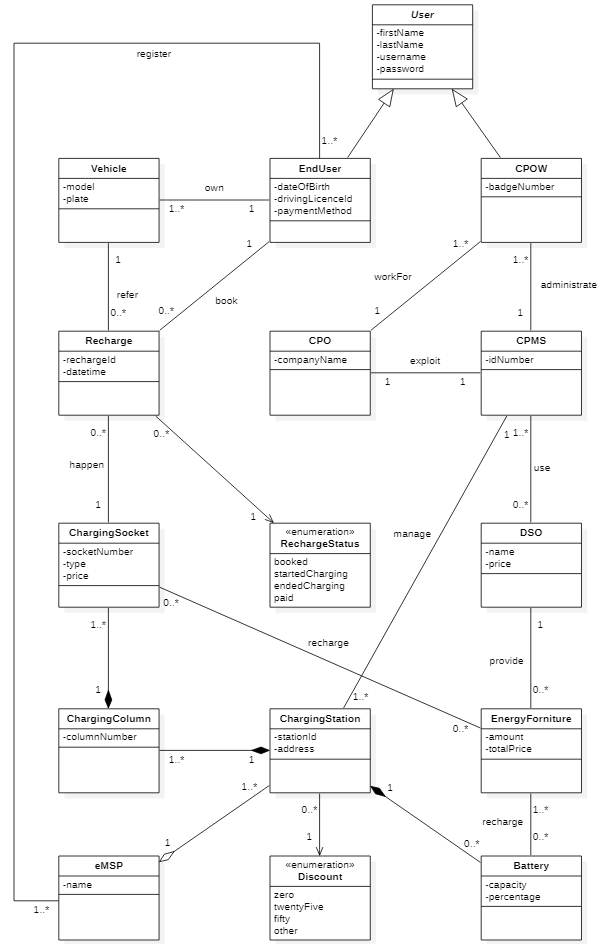
\includegraphics[width=\textwidth]{classDiagramRASDUpdated.png}
\caption{UML Class Diagram}
\label{fig:class-diagramRASD}
\end{figure}
\restoregeometry

\newgeometry{top=0.1cm}
\begin{figure}[p]
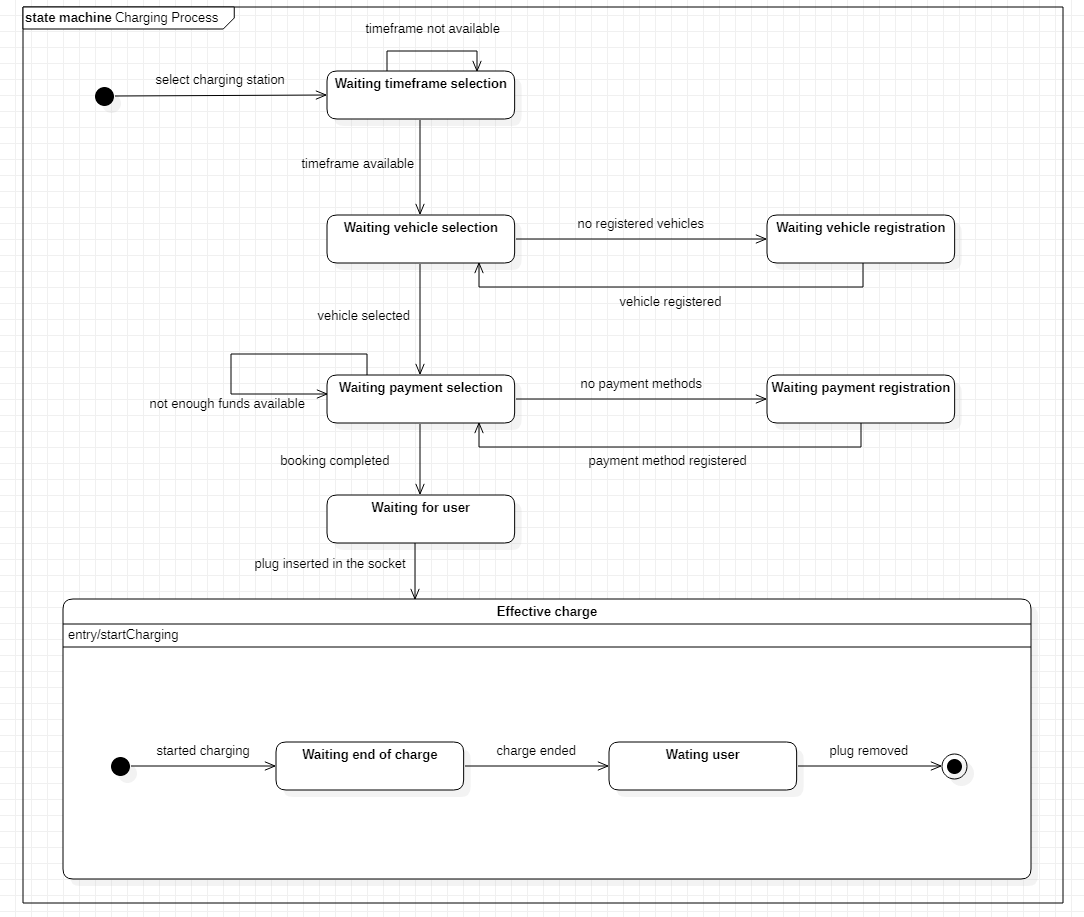
\includegraphics[width=\textwidth]{StateChartRASD}
\caption{UML State Diagram for a whole charging process}
\label{fig:state-diagramRASD}
\end{figure}

\begin{figure}[p]
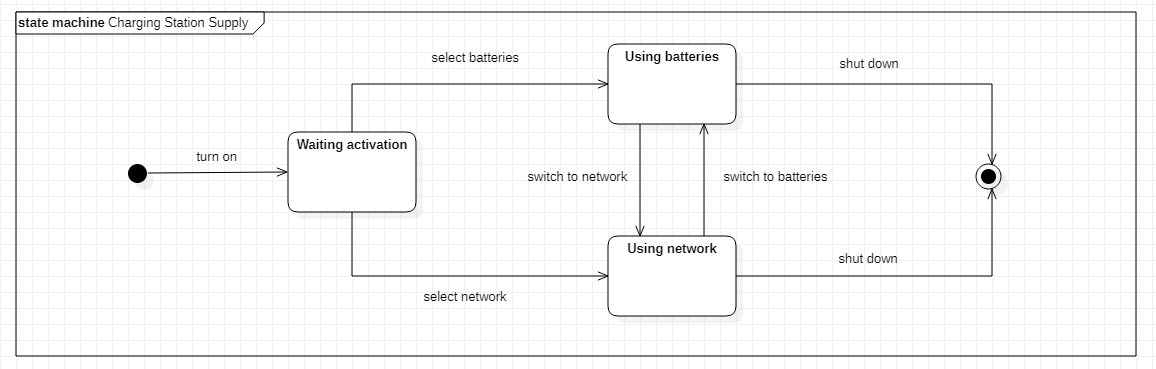
\includegraphics[width=\textwidth]{ChargingStationSupplayStateChartRASD}
\caption{UML State Diagram for Charging Station energy supply}
\label{fig:state-diagramChargingRASD}
\end{figure}
\restoregeometry

\subsubsection{Other}
Other objects are not represented in UML state charts since they don't change state at all during the system activities or the changes are too trivial to be represented in a diagram.

\section{Product functions}
In this section the most important functions that the eMall app will offer are presented divided by the type of user that will exploit them.

\subsection{Unregistered user}

\subsubsection{Application exploring}
When a user in not logged-in into the application the system will show a map containing the nearest charging stations and the related prices. This information can be accessed also in a list format where also some filters are available, but any operation (e.g. book a recharge) can't be performed until the login/registration.

\subsubsection{End user registration}
The system allows unregistered users to register and become effective end users of the application. They have to provide their first name, last name, username, password, date of birth and driving license ID. All these fields are mandatory in order to complete successfully the registration process. Optionally a user will be able to register a car and a payment method during the registration process, but this operation can also be performed later.

\subsubsection{CPOW registration}
The system allows newly hired CPOWs to set up their accounts in order to access the CPMS management web interface. They have to provide their first name, last name, username, password, and most important thing, their badge number. Also in this case, all fields are mandatory in order to complete successfully the registration process, otherwise, it will fail.

\subsection{Authenticated end user}
Here the focus is on the purpose of eMall on the end user side. In particular, we have two main functionalities.
\subsubsection{Charge booking}
The booking of a charge is the most important function that coincides with the main purpose of the whole system on the end user side. When a user is logged in, the system shows a map with all the nearest charging stations and lets the user navigate through them and sees current prices for different types of sockets of the different stations. Furthermore, the system will inform the user about special discounts and offers.

Once the user has selected a charging station and a date the system will show him all the available time frames and will allow completing the booking only if both a vehicle and a payment method with enough funds have been correctly selected. In all the other cases the operation couldn't be completed correctly.

\subsubsection{Charging process}
The system must manage also the whole charging process. So, when a user presses the charge button on the app and connects his car to the booked charging socket, the system will start dispensing energy to the car. All the process will be monitored by the system and the app will display to the user the remaining time and will send a notification to him once the process will be ended. At this point, the system will charge the import of the whole recharge on the payment method of the user.

\subsection{Authenticated CPO worker}
Now let's put focus on the CPO side.
\subsubsection{Selecting from which DSO acquire energy}
In normal execution, DSOs are selected dynamically by the system, trying to exploit the best quality/spent agreement based on prices and dates of different companies.

But can happen that a CPOW needs to manage the selection through his web interface. When he enters the related section, the system will show him a list of all the charging stations and for each one of them a list of DSOs available in that specific geographical area and their prices, with the possibility to turn off the auto-deciding process for each one of the stations and manually select a new DSO.
\subsubsection{Charging station energy management}
Also charging station use of energy in normal execution is managed dynamically by the system. In this case, the focus is to use batteries in order to exploit price swings in trying to reach the best level of revenue (e.g. when the energy price is low the system will use energy directly from the DSO to charge vehicles and recharge also batteries. On the other hand when the energy price increase over a certain threshold the system will, first of all, consume all energy in batteries bought at lower prices before acquiring new).

Also in this case a CPOW can, always through his web interface, go to the related section. The system will show him a list of all the charging stations and for each one of them, there is the possibility to set the price threshold or to directly manually manage the use of batteries or directly of the network.
\subsubsection{Show charging station status}
The system will also allow CPOWs to know both the internal and external status of each charging station. When a CPOW access the related section on the web interface a list of all charging stations related to his CPO is shown. By clicking on one of them the station structure is shown (e.g. number of sockets and their types). Also current status is visible, so the list of both currently happening charges and booked charges are shown, with all the informations related to the interested vehicles.


\section{User characteristics}
The system has the following different types of users:
\begin{itemize}
\item \textit{Unlogged End User}: an unlogged user of the system can see charging stations near his position on the map and their prices but he can't do any type of operation (i.e. booking a charge). He can change his status by registering to the service or logging in as \textit{End User}.
\item \textit{End User}: is the main user of the system that can register vehicles, add payment methods, exploit special offers, and book and complete vehicle charges.
\item \textit{Unlogged CPOW}: an unlogged CPOW can only see the registration/log-in interface on the web interface but won't be able to perform any kind of operation. He can change his status by registering or logging in as a CPOW.
\item \textit{CPOW}: an operator which is related to a \textit{CPMS} through which he can manage different charging stations (i.e. deciding to supply sockets from batteries or directly from the network), see \textit{DSO} offers and manually decide from which of them purchase energy supplies.

\end{itemize}


\section{Assumptions, dependencies and constraints}

\subsection{Domain assumptions}

In the following rows domain assumptions are presented:
\begin{itemize}
\item{[D1]} \label{D1} Each CPO is associated with one and only one CPMS.
\item{[D2]} \label{D2} All charging stations have been already correctly added in the right coordinates to third party map used.
\item{[D3]} \label{D3} An End User can't disconnect the plug during the charging process.
\item{[D4]} \label{D4} A unique identifier has been associated physically to every charging station.
\item{[D5]} \label{D5} CPOs must manage their charging station only through his related CPMS.
\item{[D6]} \label{D6} Energy can't be supplied by different DSOs at the same time to the same charging station.
\item{[D7]} \label{D7} Each charging socket can't be supplied by both batteries and the network at the same time.
\item{[D8]} \label{D8} Every end user make charges at the charging station with the specific vehicle he has booked for.
\item{[D9]} \label{D9} The networks that allows the energy furniture from DSOs to charging sockets or batteries must work properly.
\item{[D10]} \label{D10} The system exploits APIs to retrieve information about energy prices from different DSOs.
\item{[D11]} \label{D11} Charging sockets are equipped with an \textit{RFID} receiver in order to be unlocked.
\end{itemize}
\subsection{Dependencies and constraints}
Some third-party applications and dates from public institutions are necessary to make all functionalities of the system work properly.
\begin{itemize}
    \item \textit{Vehicle registering check}: check if inserted car model and plate exists.
    \item \textit{Vehicle model information get}: get dates of all the electric vehicle models in commerce in order to know in advance which is the maximum battery capacity for each booked charge.
    \item \textit{Payment method check}: check if the payment method added by the user works properly. It will be exploited also before every charge starts in order to ensure that on the payment method there are enough funds to complete a full charge.
    \item \textit{Map service}: exploit a map service to show a map with all charging stations in the application.
\end{itemize}

\chapter{Specific Requirements}
\section{External Interface Requirements}
\subsection{User Interfaces}
eMall provides two different types of user interfaces, one for each type of user. In detail, end users exploit provided services through a mobile application, absolutely necessary to unlock charging sockets and start the charging process. On the other hand, CPOWs, which are meant like normal office workers, exploit their managing functionalities through a web application. Both interfaces have to satisfy accessibility requirements and, in particular, the mobile application must be user-friendly. The goal is e-mobility for all, so also older people with low technological skills must be able to perform all required operations to book and complete a charge.
\subsection{Hardware Interfaces}
Since eMall is a software system, no specific hardware interfaces are provided to users. But clearly, end users will interact with charging station hardware (i.e. RFID receivers of charging sockets) that are already provided by domain assumptions. So the communication hardware of the mobile phone on which the mobile up runs is exploited.
\subsection{Software Interfaces}
Since no other applications need to retrieve any kind of data from eMall there are no software interfaces provided. But, like for Hardware Interfaces, the system exploits third-party software as reported in the dependencies section and also other APIs for information retrieval (e.g. DSOs prices) as declared in the domain assumption section.
\subsection{Communication Interfaces}
The whole eMall service is based on communication between different actors. Both the mobile app and CPMS communicate with the central eMall server through uniform internal APIs exploiting HTTPS protocol. In either the two subsystems type of communication is bidirectional, they need to send and receive data from the central server. For example, the mobile app must get updated availabilities of free charging slots but also update the central server when a booking is made. On the other side, also CPMS must always get updated information from the server, but also set, for example, a new DSO for a certain charging station.

Also communication with all the charging stations is necessary. In detail, the main server communicates with charging stations always through internal uniform APIs. Furthermore, RFID technology is exploited to allow communication between the mobile app and the charging socket (i.e. for unlocking the charging socket). In particular, mobile phones communicate with the RFID receiver of the sockets.

All other types of communication, like the one with all third-party software presented in the dependencies section, happen through API, as the retrieval of DSOs prices.



\section{Functional Requirements}
\begin{itemize}
    \item{[R1]} \label{R1} The system must allow unregistered/registered users to see a map of available charging stations and their prices and offers.
    \item{[R2]} \label{R2} The system must allow unregistered/registered users to see a list of charging stations and filter on it (e.g. offers, prices and positions).
    \item{[R3]} \label{R3} The system must allow unregistered users to register as end user or CPOW (if they have a badge id).
    \item{[R4]} \label{R4} The system must verify if the all data inserted by users are correct (e.g. personal data, vehicle and payment method information, charging station ID).
    \item{[R5]} \label{R5} The system must allow registered end users or CPOW to log in through their username and password.
    \item{[R6]} \label{R6} The system must allow registered end users to associate vehicles to their account and keep track of them.
    \item{[R7]} \label{R7} The system must allow registered end users to associate payment methods to their account.
    \item{[R8]} \label{R8} The system must allow registered end users to view the available time-slots for a certain type of socket of a certain charging station in a specific day.
    \item{[R9]} \label{R9} The system must allow registered end users to book a charge in a specific charging station.
    \item{[R10]} \label{R10} The system must allow end users to unlock a charging socket if they have booked it and it's the correct time-slot.
    \item{[R11]} \label{R11} The system must let a charge start if a vehicle is correctly connected and the charging socket is unlocked.
    \item{[R12]} \label{R12} The system must show to end users the charging status (e.g. remaining time to complete charge).
    \item{[R13]} \label{R13} The system must notify the end-user when the charge is complete.
    \item{[R14]} \label{R14} When a charging process is correctly finished the system must charge on the end user selected payment system the correct import.
    \item{[R15]} \label{R15} The system must allow CPOW to register a new charging station through its physical id.
    \item{[R16]} \label{R16} The system must be able to dynamically select if using batteries, directly the network or a mix of the two for each charging station.
    \item{[R17]} \label{R17} The system must allow CPOWs to manually select if using batteries, directly the network or a mix of the two for each charging station associated to them.
    \item{[R18]} \label{R18} The system must be able to dynamically select which DSO use to provide energy to a specific charging station.
    \item{[R19]} \label{R19} The system must allow CPOWs to manually select which DSO use to provide energy to a specific charging station associated to them.
    \item{[R20]} \label{R20} The system must be able to dynamically decides if a certain energy furniture is destinated to a battery or directly to sockets of charging stations .
    \item{[R21]} \label{R21} The system must allow CPOWs to manually decides if a certain energy furniture is destinated to a battery or directly to sockets of charging stations associated to them.
    \item{[R22]} \label{R22} The system must keep track of the current status of each charging process (e.g. booked, startedCharging, etc.).
    \item{[R23]} \label{R23} The system must keep track of the structure of each charging station (e.g. number of columns, number and type of sockets).
    \item{[R24]} \label{R24} The system must allow CPOWs to view the structure of each charging station associated to them.
    \item{[R25]} \label{R25} The system must keep track for each charging station of all bookings related to it.
    \item{[R26]} \label{R26} The system must allow CPOWs to view all the bookings of a certain charging station associated to them and their status.
    \item{[R27]} \label{R27} The system must allow CPOWs to set prices and special offers for a certain charging station associated to him.
\end{itemize}

In the following table is shown which Domain Assumptions and Requirements are involved for each goal.
\begin{table}[H]
  \centering
  \begin{tabular}{|c|c|c|c|}
    \cline{2-3}
    \multicolumn{1}{c|}{} & Domain Assumptions  & Requirements \\ \hline
    G1 & D2 & R1 R2 R8\\ \hline
    G2 & D3 D8 D9 D11 & R3 R4 R5 R6 R7 R9 R10 R11 R12 R13 R14\\ \hline
    G3 & D1 D4 D5 D6 D7 D11 & R5 R15 R16 R17 R20 R21 R22 R23 R24 R25 R26 R27\\ \hline
    G4 & D9 D10 & R5 R18 R19 \\ \hline
  \end{tabular}
  \caption{Correspondence between Domain Assumptions and Requirements and Goals}
\end{table}

\subsection{Use cases}
In this section the various use cases present in the use case diagram and derived from the scenarios previously described are illustrated in detail.\\ \\
\phantomsection
\textbf{1. Registration}\label{uc:1}
\\
\\
Actors: Non registered End-User or CPOW\\ \\
Entry condition:
\begin{itemize}
\item The End-User/CPOW does not have an account and has the application/web interface opened
\end{itemize}
Flow of events:
\begin{itemize}
\item The End-User/CPOW clicks on the "Login or Register" button.
\item The End-User/CPOW clicks on the "Register" button.
%\item The End-User/CPOW clicks on the "I'm a User"/"I'm a CPOW" button.
\item The End-User/CPOW provides name, surname, date of birth, email address, all information about his debit card and all information about his electric vehicles that he wants to register/the associated ID of the CMPS where he works and a special code provided by his employer.
\item The End-User/CPOW provides username and password.
\item The End-User/CPOW clicks on the “confirm” button.
\end{itemize}
Exit conditions:
\begin{itemize}
\item A successful message is sent to the User which is redirected to the main page of the account
\end{itemize}
Exceptions:
\begin{itemize}
\item The personal information are not correct. The system shows an error message and asks the End-User to re-write the incorrect ones.
\item Debit Card information are not correct. The system shows an error message and asks the End-User to re-write the incorrect ones.
\item Electric vehicle information are not correct. The system shows an error message and asks the End-User to re-write the incorrect ones.
\item The CMPS ID is incorrect or doesn't exists. The system shows an error message and asks the CPOW to re-write it.
\item The username was already taken by another user. The system shows an error message and asks the End-User to choose another username.
\item The End-User interrupts the registration process clicking to "exit" button. He's redirected to the main page
\end{itemize}
\phantomsection
\textbf{2. Log in}\label{uc:1}
\\
\\
Actors: Registered End-User or CPOW\\ \\
Entry condition:
\begin{itemize}
\item The End-User/CPOW has the application/web service opened
\end{itemize}
Flow of events:
\begin{itemize}
\item The End-User/CPOW clicks on the "Login or Register" button.
\item The End-User/CPOW inserts username and password.
\item The End-User/CPOW clicks on the “Login” button.
\end{itemize}
Exit conditions:
\begin{itemize}
\item The End-User/CPOW is redirected to the main page of the account
\end{itemize}
Exceptions:
\begin{itemize}
\item Username and/or Password are/is incorrect. The system shows an error message and asks the End-User to re-write it.
\end{itemize}
\phantomsection
\textbf{3. Non Registered End-User charging stations map view}\label{uc:1}
\\
\\
Actors: Non registered End-User\\ \\
Entry condition:
\begin{itemize}
\item The End-User does not have an account and has the application opened
\end{itemize}
Flow of events:
\begin{itemize}
\item The End-User clicks on the "Browse Map" button.
\item A map with all nearby charging station each with a price review is displayed.
\item The End-User clicks on a charging station in the map.
\item A short description of that charging station is displayed (including price and special offers).
 account.
\end{itemize}
Exit conditions:
\begin{itemize}
\item A summary of that charging station is displayed (including price and special offers). If the End-User tries to book a charge with the "book a charge" button the system asks him to login or register.
\end{itemize}
Exceptions:
\begin{itemize}
\item No exceptions for this particular use case
\end{itemize}
\phantomsection
\textbf{4. End-User charge booking}\label{uc:4}
\\
\\
Actors: End-User \\ \\
Entry condition:
\begin{itemize}
\item Registered End-User opened the app and logged in.
\end{itemize}
Flow of events:
\begin{itemize}
\item The End-User clicks on "browse map" button.
\item A map with all nearby charging station each with a price review is displayed.
\item The End-User clicks on a charging station in the map.
\item A short description of that charging station is displayed (including price and special offers).
\item The End-User clicks on "book a charge" button.
\item The End-User selects a Day and a type of a socket.
\item The End-User selects one of the free time-slots available.
\item The End-User selects an electric vehicle associated to his account.
\item The End-User selects the amount of charge in percentage.
\item A summary of the booking is displayed.
\item The End-User clicks on the "Confirm" button.
\end{itemize}
Exit conditions:
\begin{itemize}
\item A successful message which presents the summary of the booking with in particular the number of associated charging column, number of associated socket and the booking id is sent to the End-User.
 \end{itemize}
Exceptions:
 \begin{itemize}
 \item There are no socket of that type available for that day. The system shows an error message and asks the End-User to change the date.
 \item The End-User interrupts the booking process clicking to "exit" button. He's redirected to the charging stations map.
\end{itemize}
\phantomsection
\textbf{5. End-User benefits from a special offer from the list panel}\label{uc:5}
\\ \\
Actors: End-User \\ \\
Entry condition:
\begin{itemize}
\item Registered End-User opened the app and logged in.
\end{itemize}
Flow of events:
\begin{itemize}
\item The End-User clicks on "browse map" button.
\item The End-User clicks on "list charging stations" button.
\item The End-User selects a Day, a type of a socket, a price range and an order.
\item All charging stations with a socket type of the selected one available in the selected Day and with a price included in the price range selected are displayed in the right order.
\item The End-User selects a certain charging station.
\item The End-User selects one of the free time-slots available.
\item The End-User selects an electric vehicle associated to his account.
\item The End-User selects the amount of charge in percentage.
\item A summary of the booking is displayed.
\item The End-User clicks on the "Confirm" button.
\end{itemize}
Exit conditions:
\begin{itemize}
\item A successful message which presents the summary of the booking with in particular the number of associated charging column, number of associated socket and the booking id is sent to the End-User.
 \end{itemize}
Exceptions:
 \begin{itemize}
 \item There are no charging stations that satisfies the searching conditions. The search result is empty.
 \item The End-User interrupts the booking process clicking to "exit" button. He's redirected to the main charging stations list page
\end{itemize}
\phantomsection
\textbf{6. End-User vehicle charging}\label{uc:7}
\\ \\
Actor: End-User \\ \\
Entry condition:
\begin{itemize}
\item The End-User has previously booked a charge and now is at the charging station near the associated charging column with his vehicle. He has opened the application and logged in.
\end{itemize}
Flow of events:
\begin{itemize}
\item The End-User clicks on "my Bookings" button.
\item All available charge bookings are displayed.
\item The End-User selects one of those
\item The End-User clicks on "unlock charging column" button.
\item A successful message is displayed and the associated socket of the booked charging column became available.
\item The End-User connects his vehicle to the socket.
\item The charging process starts automatically and the application displays progressively the amount of charge done.
\item When the booked amount of charge is reached the charging process stops and the application displays a message.
\item The End-User disconnects the vehicle from the socket.
\item The used socket of the charging column is blocked.
\item The End-User clicks on "end charge" button.
\end{itemize}
Exit conditions:
\begin{itemize}
\item The system elaborates the payment and displays a successful message to the End-User.
\end{itemize}
Exceptions:
\begin{itemize}
\item The End-User has arrived too late and the booking has been expired. The system shows an error and deletes the booking.
\item The End-User has arrived too early respects to the time-slot of the booking and is not able to click on "unlock charging column" button.
\item The charging process cannot be doing correctly. The system shows an error message, displays a list of possible solutions to solve the problem.
\item The payment has not been successful. The system shows an error message indicating that the balance is still to be paid and displays a list of possible solutions to solve the problem.
\end{itemize}
\phantomsection
\textbf{7. CPO charging station registration}\label{uc:1}
\\
\\
Actors: Registered CPOW\\ \\
Entry condition:
\begin{itemize}
\item Registered CPOW opened the app and logged in.
\end{itemize}
Flow of events:
\begin{itemize}
\item The CPOW clicks on the "Charging Stations" button.
\item The CPOW clicks on the "New Charging Station" button.
\item The CPOW provides charging station name, position and physical ID.
\item The CPOW clicks on the “confirm” button.
\end{itemize}
Exit conditions:
\begin{itemize}
\item A successful message is sent to the CPOW
\end{itemize}
Exceptions:
\begin{itemize}
\item Charging station information are incorrect or it doesn't exists. The system shows an error message and asks the CPOW to re-write it.
\item The CPOW interrupts the registration process clicking to "exit" button. He's redirected to the main page
\end{itemize}
\phantomsection
\textbf{8. CPO energy acquiring from DSO}\label{uc:8}
\\ \\
Actor: Registered CPOW \\ \\
Entry condition:
\begin{itemize}
\item Registered CPOW opened the app, logged in.
\end{itemize}
Flow of events:
\begin{itemize}
\item The CPOW clicks on "View DSOs Offers" button.
\item A list of all DSOs offers is displayed.
\item The CPOW clicks on a certain DSO offer.
\item A page with all information about that offer is displayed.
\item The CPOW clicks on "Acquire energy from this DSO".
\item The CPOW clicks on "Confirm" button.
\end{itemize}
Exit conditions:
\begin{itemize}
\item The system displays a successful message to the CPOW.
\end{itemize}
Exceptions:
\begin{itemize}
\item Energy can't be acquired by that DSO for the selected charging station. The system shows an error message to the CPOW and displays a list of possible solutions to solve the problem.
\item The CPOW interrupts the process clicking to "exit" button. He's redirected to the main page of the account.
\end{itemize}
\phantomsection
\textbf{9. CPO batteries management}\label{uc:8}
\\ \\
Actor: Registered CPOW \\ \\
Entry condition:
\begin{itemize}
\item Registered CPOW opened the app, logged in.
\end{itemize}
Flow of events:
\begin{itemize}
\item The CPOW clicks on "Charging Stations" button.
\item A list of all associated charging stations is displayed.
\item The CPOW clicks on one of those.
\item A page with all features of the selected charging station is displayed (e.g "internal" and "external" status, all bookings associated ).
\item The CPOW clicks on "Batteries Management".
\item A list of all batteries associated to that charging station is displayed.
\item The CPOW clicks on one of those.
\item A page with all features about that battery is displayed.
\item The CPOW clicks on "Store energy" button.
\end{itemize}
Exit conditions:
\begin{itemize}
\item The system starts the energy storing process and then shows a successful message to the CPOW.
\end{itemize}
Exceptions:
\begin{itemize}
\item There are no charging stations available. The systems shows a message which says that
the list is empty.
\item The are no available batteries. The systems shows a message which says that the list is empty.
\item The are no available DSO agreements for the selected charging station. The systems shows an error message.
\item The energy storing process doesn't work properly. The system stops it, shows an error message to the CPOW and displays a list of possible solutions to solve the problem.
\end{itemize}
\phantomsection
\textbf{10. CPO energy supply}\label{uc:8}
\\ \\
Actor: Registered CPOW \\ \\
Entry condition:
\begin{itemize}
\item Registered CPOW opened the app, logged in.
\end{itemize}
Flow of events:
\begin{itemize}
\item The CPOW clicks on "Charging Stations" button.
\item A list of all associated charging stations is displayed.
\item The CPOW clicks on one of those.
\item A page with all features of the selected charging station is displayed (e.g "internal" and "external" status, all bookings associated ).
\item The CPOW clicks on "Energy Furniture" button.
\item A list of all DSOs services purchased and of all charged batteries associated is available with a brief summary of their main features for each of them are displayed.
\item The CPOW clicks on one of the DSOs services.
\item The CPOW inserts the amount of energy in percentage.
\item The CPOW clicks on "Confirm" button.
\item The CPOW is redirected to the previous list.
\item The CPOW clicks on one of the batteries.
\item The CPOW inserts the amount of energy in percentage.
\item The CPOW clicks on "Confirm" button.
\item The CPOW is redirected to the previous list.
\item The CPOW clicks on "Continue" button.
\item A summary of the total energy supply is displayed.
\item The CPOW clicks on "Confirm" button.
\end{itemize}
Exit conditions:
\begin{itemize}
\item The system starts the energy transfer process and then shows a successful message to the CPOW.
\end{itemize}
Exceptions:
\begin{itemize}
\item There are no charging stations available. The systems shows a message which says that the list is empty.
\item There are no DSO agreements and/or charged batteries available. The systems shows a message which says that the list is empty..
\item The energy transfer process doesn't work properly. The system stops it, shows an error message to the CPOW and displays a list of possible solutions to solve the problem.
\item The CPOW interrupts the process clicking to "exit" button. He's redirected to the main page of the account.
\end{itemize}
\phantomsection
\textbf{11. CPOW set a special offer}\label{uc:8}
\\ \\
Actor: Registered CPOW \\ \\
Entry condition:
\begin{itemize}
\item Registered CPOW opened the app, logged in.
\end{itemize}
Flow of events:
\begin{itemize}
\item The CPOW clicks on "Charging Stations" button.
\item A list of all associated charging stations is displayed.
\item The CPOW clicks on one of those.
\item A page with all features of the selected charging station is displayed (e.g "internal" and "external" status, all bookings associated ).
\item The CPOW clicks on "Set Special Offer".
\item The CPOW selects a type of socket, the amount of discount, a start and an end date.
\item The CPOW clicks on "Confirm" button.
\end{itemize}
Exit conditions:
\begin{itemize}
\item The system shows a successful message to the CPOW.
\end{itemize}
Exceptions:
\begin{itemize}
\item There are no charging stations available. The systems shows a message which says that the list is empty.
\item The are no available DSO agreements for the selected charging station. The systems shows an error message.
\item The CPOW interrupts the process clicking to "exit" button. He's redirected to the main page of the account.
\end{itemize}

In the following table is shown which goals are involved in every use case.
\begin{table}[H]
  \centering
  \begin{tabular}{|c|c|c|c|c|c|c|c|c|c|c|c|}
    \cline{2-12}
    \multicolumn{1}{c|}{} & UC1 & UC2 & UC3 & UC4 & UC5 & UC6 & UC7 & UC8 & UC9 & UC10 & UC11 \\ \hline
    G1 & X & X & X &  & X &  &  &  &  &  &  \\ \hline
    G2 & X & X &  & X & X & X &  &  &  &  &  \\ \hline
    G3 & X & X &  &  &  &  & X &  & X & X & X \\ \hline
    G4 & X & X &  &  &  &  &  & X &  &  &  \\ \hline
  \end{tabular}
  \caption{Correspondence between use cases and goals}
\end{table}

In the following table is shown which requirements are involved in every use case.
\begin{table}[H]
  \centering
  \begin{tabular}{|c|c|c|c|c|c|c|c|c|c|c|c|}
    \cline{2-12}
    \multicolumn{1}{c|}{} & UC1 & UC2 & UC3 & UC4 & UC5 & UC6 & UC7 & UC8 & UC9 & UC10 & UC11 \\ \hline
    R1 & X &

    X & X &  &  &  &  &  &  &  &  \\ \hline
    R2 & X & X &  &  & X &  &  &  &  &  &  \\ \hline
    R3 & X &  &  &  &  &  &  &  &  &  &  \\ \hline
    R4 & X &  &  &  &  &  &  &  &  &  &  \\ \hline
    R5 & X & X &  &  &  &  &  &  &  &  &  \\ \hline
    R6 & X & X &  &  &  &  &  &  &  &  &  \\ \hline
    R7 & X & X &  &  &  &  &  &  &  &  &  \\ \hline
    R8 & X & X & X &  & X &  &  &  &  &  &  \\ \hline
    R9 & X & X &  & X & X &  &  &  &  &  &  \\ \hline
    R10 & X & X &  & X & X & X &  &  &  &  &  \\ \hline
    R11 & X & X &  & X & X & X &  &  &  &  &  \\ \hline
    R12 & X & X &  & X & X & X &  &  &  &  &  \\ \hline
    R13 & X & X &  & X & X & X &  &  &  &  &  \\ \hline
    R14 & X & X &  & X & X & X &  &  &  &  &  \\ \hline
    R15 & X & X &  &  &  &  & X &  &  &  &  \\ \hline
    R16* &  &  &  &  &  &  &  &  &  &  &  \\ \hline
    R17 & X & X &  &  &  &  & X & X & X & X &  \\ \hline
    R18* &  &  &  &  &  &  &  &  &  &  &  \\ \hline
    R19 & X & X &  &  &  &  & X & X &   & X &  \\ \hline
    R20* &  &  &  &  &  &  &  &  &  &  &  \\ \hline
    R21 & X & X &  &  &  &  & X & X & X & X &  \\ \hline
    R22* &  &  &  &  &  &  &  &  &  &  &  \\ \hline
    R23* &  &  &  &  &  &  &  &  &  &  &  \\ \hline
    R24 & X & X &  &  &  &  & X &  &  &  &  \\ \hline
    R25* &  &  &  &  &  &  &  &  &  &  &  \\ \hline
    R26 & X & X &  &  &  &  & X &  &  &  &  \\ \hline
    R27 & X & X &  &  &  &  & X &  &  &  &  X\\ \hline
  \end{tabular}
  \caption{Correspondence between use cases and requirements}
\end{table}
*These requirements refers to the functions done automatically by the system. For this reason there are no use case related to them.
\subsection{Use cases diagrams }
In figure 3.1, 3.2 and 3.3 are reported the UML Use Case Diagrams of the Visitor, the End-User and the CPOW respectively.
\subsection{Sequence diagrams }
In figure 3.4, 3.5, 3.6, 3.7 and 3.8 are reported the UML Sequence Diagrams for the most interesting Use Cases.
\newgeometry{top=0cm}
\begin{figure}[p]
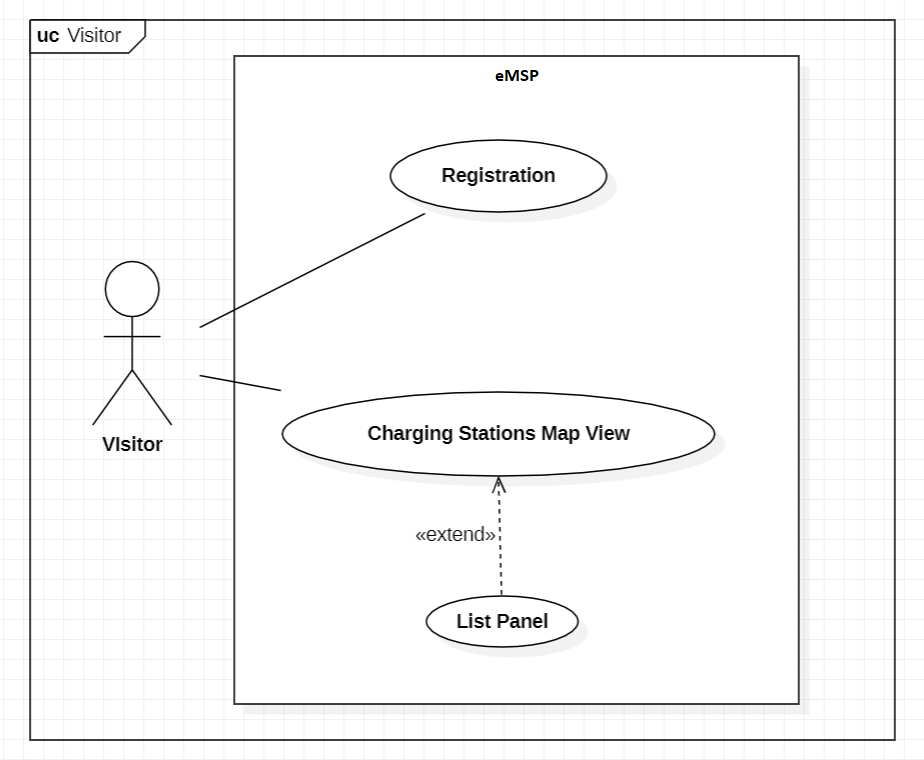
\includegraphics[width=\textwidth]{RASD/img/UC_Visitor}
\caption{Visitor UML Use Case Diagram}
\label{fig:class-diagramRASD}
\end{figure}
\restoregeometry

\newgeometry{top=0.5cm}
\begin{figure}[p]
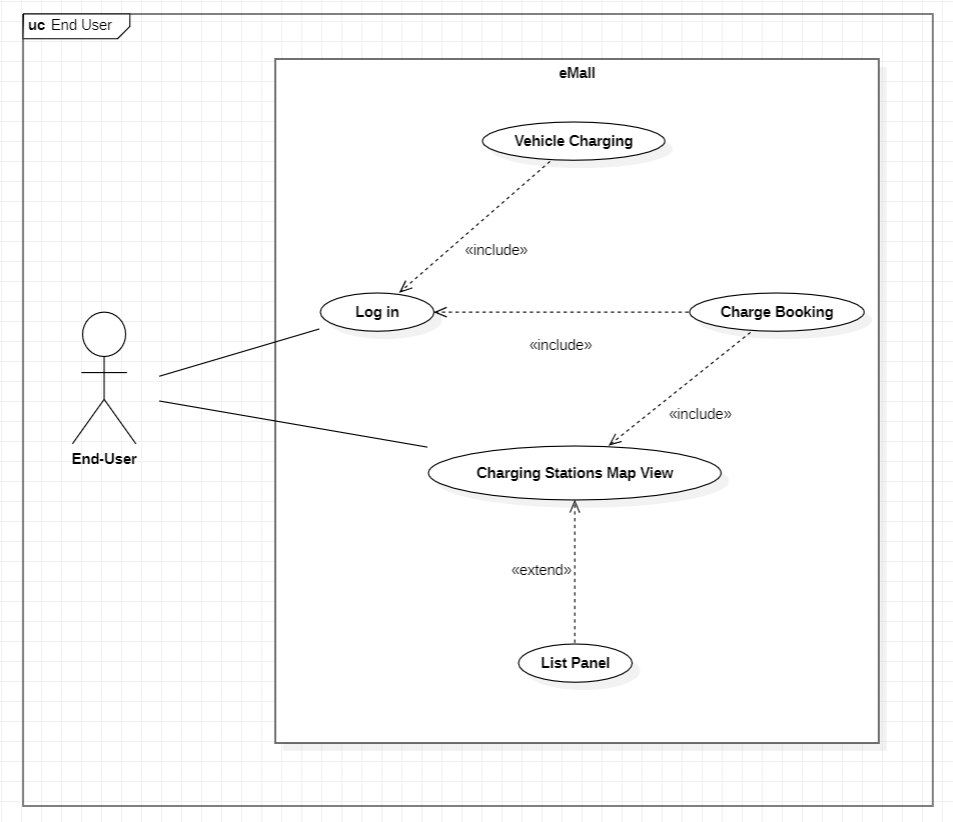
\includegraphics[width=\textwidth]{RASD/img/UC_EndUser.png}
\caption{End-User UML Use Case Diagram}
\label{fig:class-diagramRASD}
\end{figure}

\begin{figure}[p]
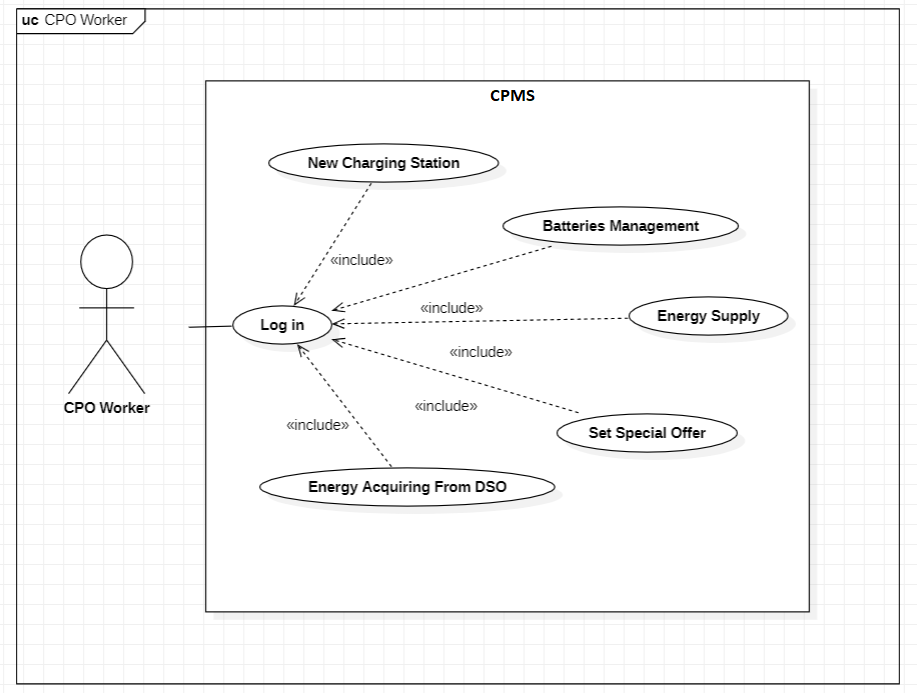
\includegraphics[width=\textwidth]{RASD/img/UC_CPOW.png}
\caption{CPOW UML Use Case Diagram}
\label{fig:class-diagramRASD}
\end{figure}
\restoregeometry



\newgeometry{top=0.5cm}
\begin{figure}[p]
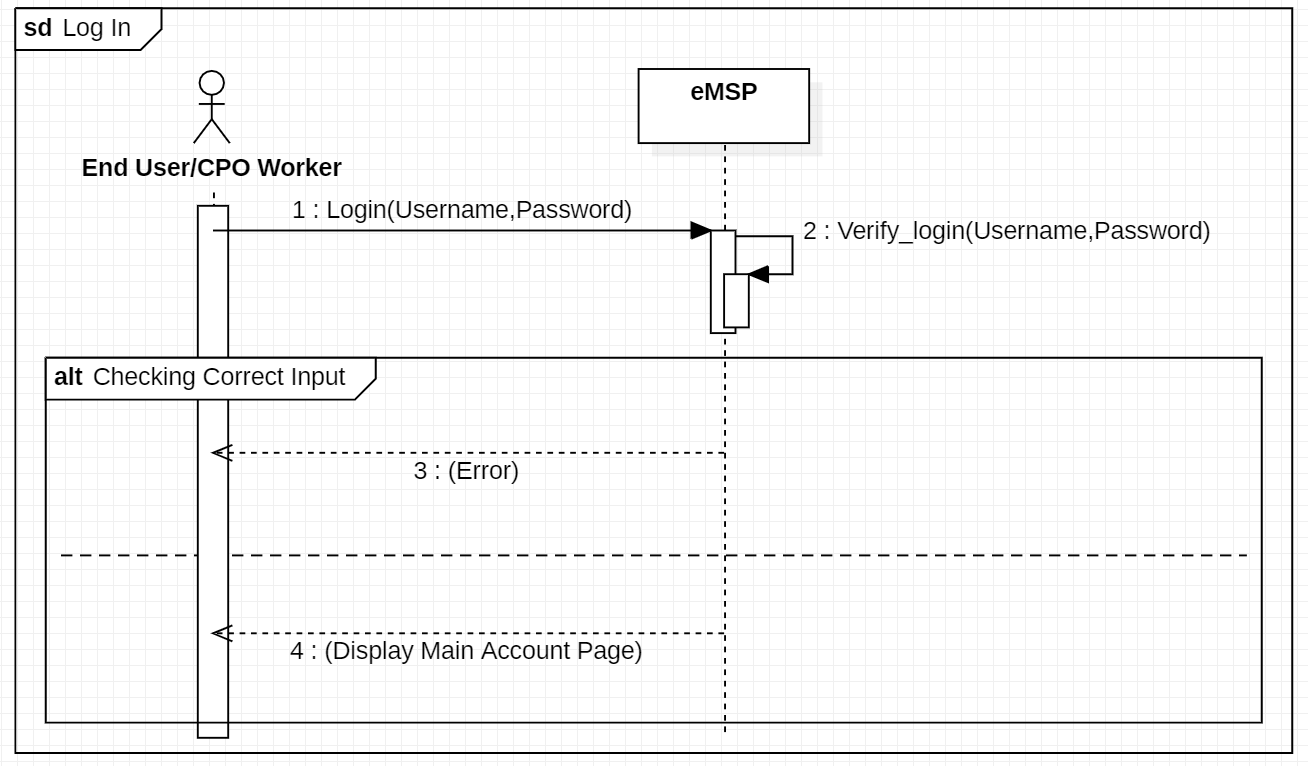
\includegraphics[width=\textwidth]{RASD/img/SD_LogIn.png}
\caption{Sequence Diagram for Use Case n° 2 (Log In)}
\label{fig:class-diagramRASD}
\end{figure}

\begin{figure}[p]
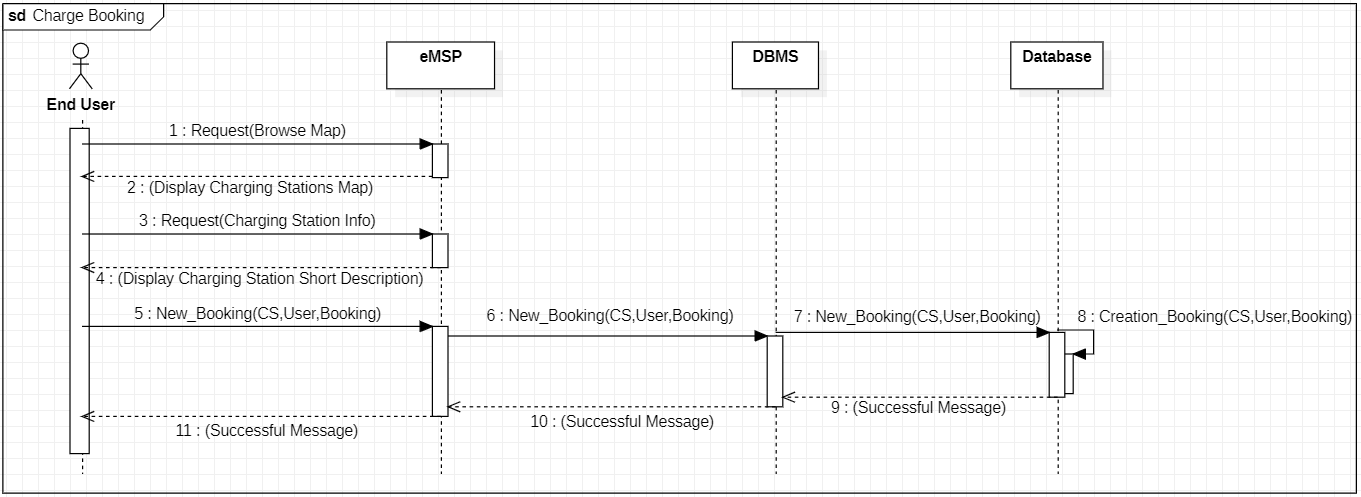
\includegraphics[width=\textwidth]{RASD/img/SD_ChargeBooking.png}
\caption{Sequence Diagram for Use Case n°4 (End-User charge booking)}
\label{fig:class-diagramRASD}
\end{figure}
\restoregeometry

\newgeometry{top=0cm}
\begin{figure}[p]
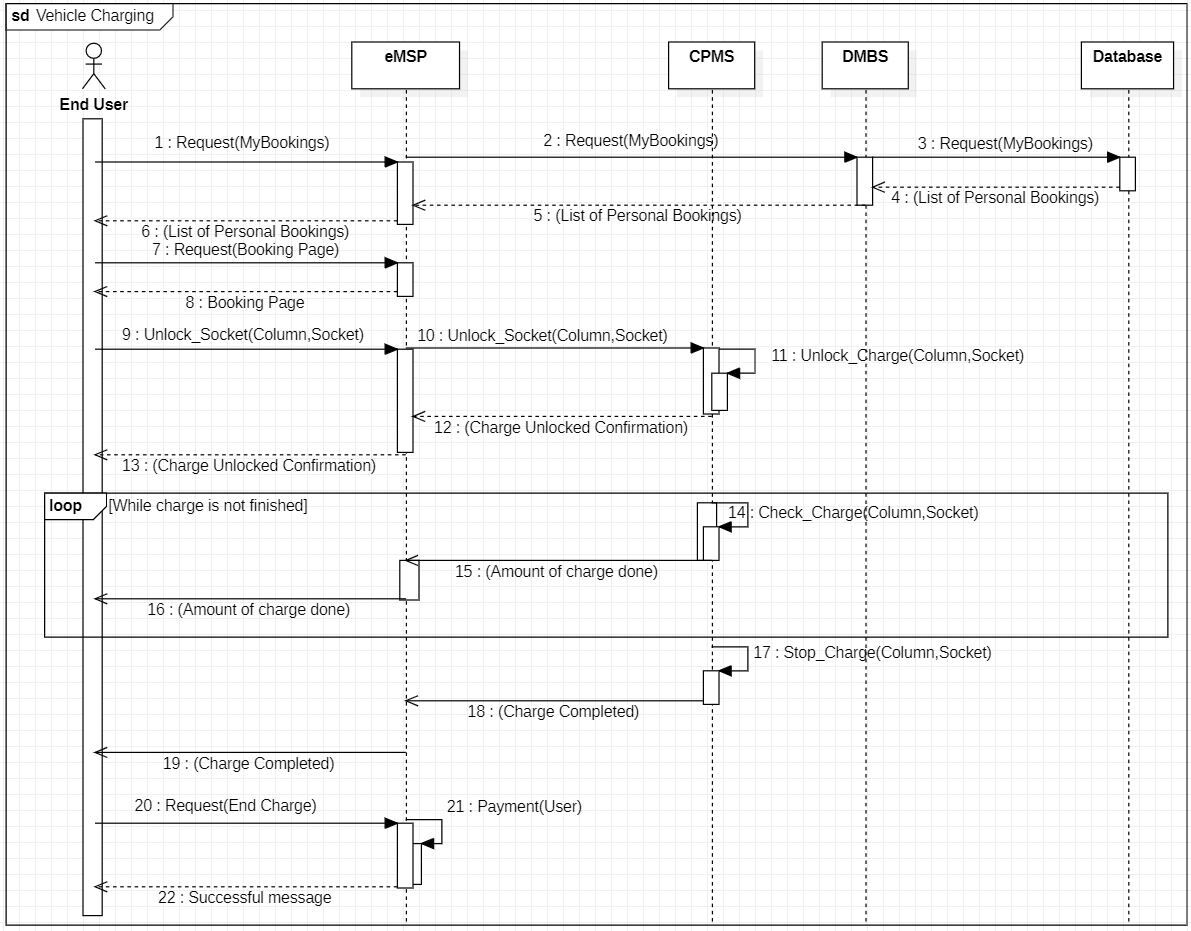
\includegraphics[width=\textwidth]{RASD/img/SD_ChargingVehicle_v2.png}
\caption{Sequence Diagram for Use Case n°6 (End-User vehicle charging)}
\label{fig:class-diagramRASD}
\end{figure}
\restoregeometry

\newgeometry{top=0.5cm}
\begin{figure}[p]
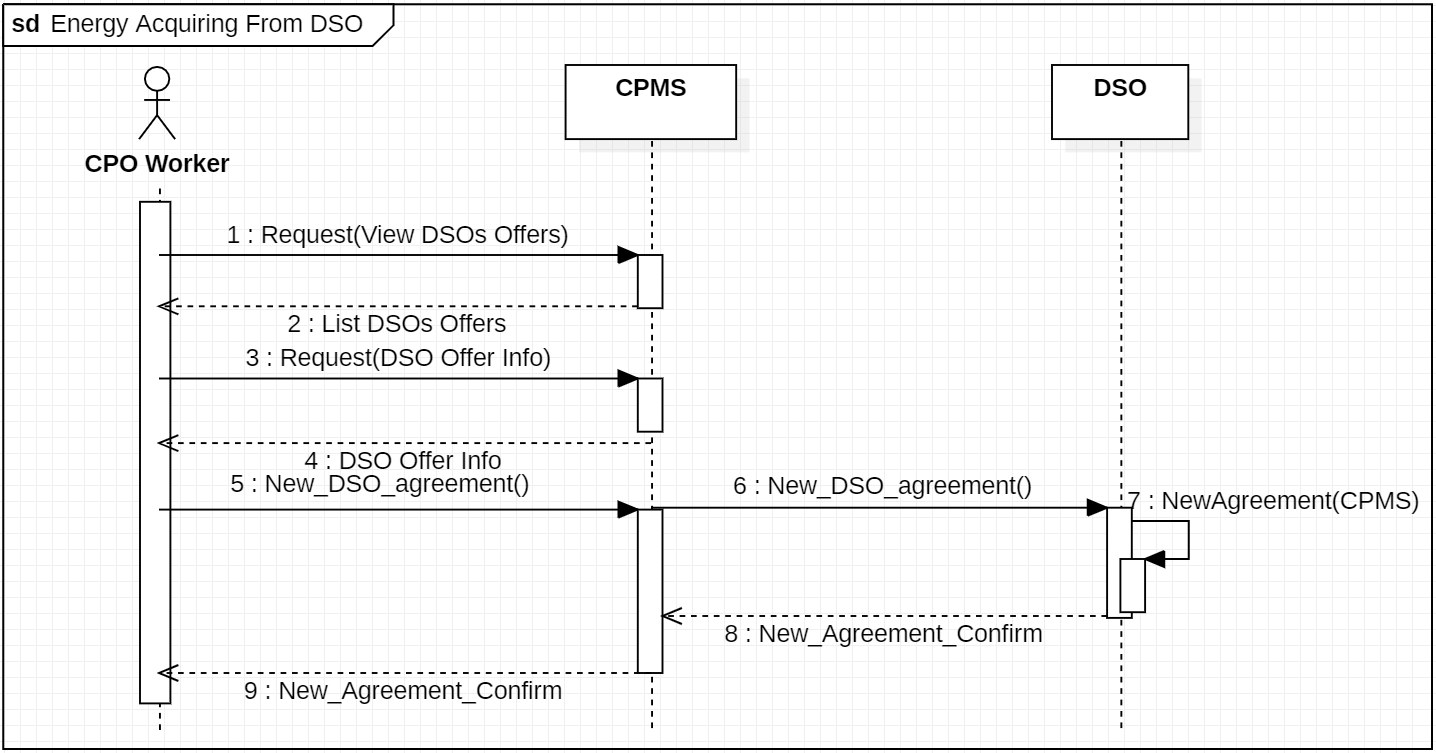
\includegraphics[width=\textwidth]{RASD/img/SD_EnergyAcquiringFromDSO_v2.png}
\caption{Sequence Diagram for Use Case n°8 (CPO energy acquiring from DSO)}
\label{fig:class-diagramRASD}
\end{figure}

\begin{figure}[p]
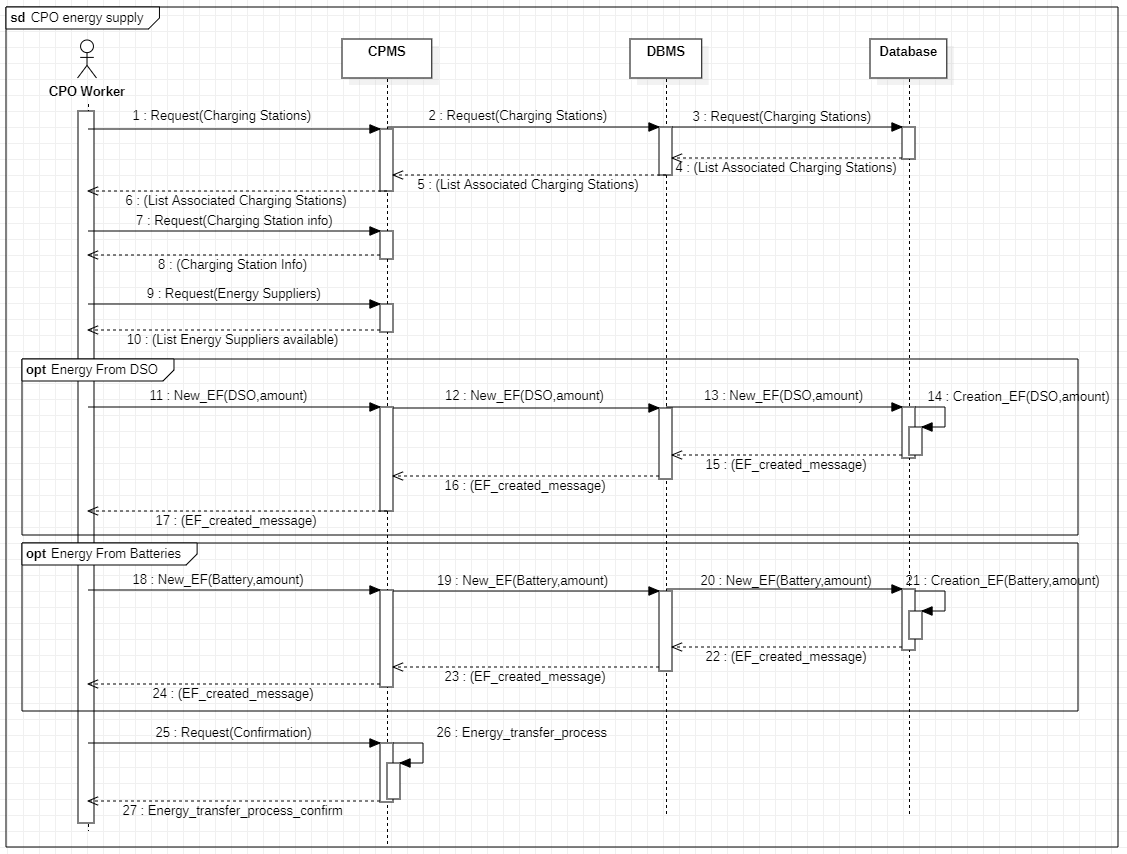
\includegraphics[width=\textwidth]{RASD/img/SD_EnergySupply_v2.png}
\caption{Sequence Diagram for Use Case n°10 (CPO energy supply)}
\label{fig:class-diagramRASD}
\end{figure}
\restoregeometry

\section{Performance Requirements}
Performances are particularly critical for eMall system. On the end user side, all operations have to be performed as fast as possible and in the correct order, e.g. overbooking of charging sockets must be avoided. Those specifications must fit also end users with low-speed internet connections. Also on the CPMS side all operations, like switching from battery power to network power, must be performed in less than 1 second. The whole computing infrastructure must be thought to be scalable, in order to allow future server capacity to increase due to the increasing number of users.

\section{Design Constraints}
\subsection{Standards compliance}
The system will only store data that are necessarily necessary to ensure the correct execution of all functionalities. The data will only be used for the purpose of eMall system and will be treated confidentially and never shared with the extern, according to European GDPR rules. In particular, the personal data of users and all information about payment methods (e.g. debit card numbers) will never be shown publicly and will be treated with the maximum level of security.

\subsection{Hardware and software limitations}
The mobile application devoted to end users usage needs the following requirements to be satisfied:
\begin{itemize}
    \item \textbf{Hardware}:
        \begin{itemize}
            \item The mobile phone of end users must support RFID communication protocol in order to be able to unlock the charging sockets.
            \item Also a GPS is necessary to show the map of near charging stations.
            \item The device must be connected to an internet connection in order to be able to perform any operation.
        \end{itemize}
    \item \textbf{Operating system}: since the main purpose of the system is e-mobility for \textbf{all}, the mobile application will be compatible also with older smartphones and minimum requirements are set quite low.
        \begin{itemize}
            \item Android 5.0 (Lollipop)
            \item iOS 9.0
        \end{itemize}
\end{itemize}
On CPOW side there aren't particular limitations since the web interface can be accessed from every device with an internet connection through every currently used web browser.

\section{Software System Attributes}
\subsection{Reliability}
The system must have the highest reliability possible since all booked recharge must be performed correctly by end users. Furthermore, the updated status of each charging station must be always known by CPMS. Based on these assumptions multiple instances of data must be available in more than one place in order to satisfy those requirements.

\subsection{Availability}
Also availability is a particularly critical requirement for the system for pretty much the same motivation of reliability. In particular, the system will guarantee 99,999\% of up-time. In other words only 5 minutes of downtime per year.

\subsection{Security}
Security is a critical requirement of this system too. The main reasons are the fact that personal data are treated (e.g. identities of users, their cars, and possibly their position if they are going to have a recharge at a specific moment) and also sensible information about payment methods (e.g. bank ID or debit card numbers). All communications between different parts of the system must be properly encrypted and also communication with external APIs must be under strict control. Furthermore, also places where data are stored must be secured and possible theft of personal data must be prevented.

\subsection{Maintainability}
The system will be implemented following coding patterns and specific software engineering practices, all accurately documented, in order to ensure fast and easy maintenance and consequently increment also availability and contribute to downtime reduction as much as possible.

\subsection{Portability}
As already mentioned, the main purpose of the system is e-mobility for \textbf{all}, so since compatibility with old devices is already guaranteed on the end user side, here there is the condition that the system is meant to be compatible also with future developed operating systems and devices as long as it will be possible. On the CPOWs side, the system will be compatible with all modern web browsers and the compatibility will be extended also to the one that will be developed in the future.

\chapter{Formal Analysis using Alloy}
The purpose of this chapter is to show, through alloy, a formal analysis of the most important aspects which characterize the whole eMall system. The scope is to define and highlight all the constraints that are absolutely necessary to make the system works properly. All the classes of the class diagram have a correspondence with alloy signatures and also the \textit{enumerations}, which represents the state of a charge (e.g. booked, paid, ..) and the type of a discount, have been modeled. Also some simplifications have been done, i.e. for the representation of time instants the \textit{Time} type of alloy has been used, but for sure it hasn't the same power and clearness of \textit{timestamp} or \textit{datetime} types from high-level programming languages. Some facts have been used to ensure that the most important constraints and requirements are satisfied, as can be seen from the diagrams reported below. In the end, some predicates have been exploited to represent the most important functionalities provided by the system and to generate some simple example worlds. In the following section, all the alloy code is shown and after, some worlds are described, in order to allow easy comprehension of how the system will work.
\section{Alloy Code}
\lstinputlisting[language=alloy]{alloy.als}

\section{Worlds}
We decided to represent three different worlds to give a presentation on the most important aspect of eMall system.

\subsection{First world}
In the first world, the focus is on the end-user and on the recharge process, as can be seen from figure \ref{fig:world1}. To provide a better clean report we decided to hide the CPO subsystem in order to focus only on the end-user. As can be observed from the picture two end-users that book two different recharge are the main actors. There are two different charging sockets of two different charging columns belonging to the same charging station. The two recharges are on the same charging socket in two different timeframes and users already paid for both. The most important checked constraints are:
\begin{itemize}
    \item Only end users with a registered vehicle can be associated with a recharge.
    \item Only end users with a registered payment method can be associated with a recharge. In that specific case, we see that the different users used the same payment method. This is a kind of situation that can happen. E.g. the two users are a wife and a husband and decided to pay with the same debit card. This assumption can be supported by the fact that the two recharges are consecutive (one starts when the other end) so they might be together with their two electric cars.
    \item The target vehicle of each recharge must be associated with the end user who books the recharge.
    \item More recharges can't happen in the same socket at the same time.
    \item Status must be coherent (e.g. a recharge scheduled after another can't be paid if the other one is still booked).
    \item Charging sockets belongs to only one charging column that belongs to only one charging station.
\end{itemize}

\subsection{Second world}
In the second world, we move our focus on the CPO subsystem, as can be seen in figure \ref{fig:world2}. Also in this case, to provide a cleaner report users and recharges have been hidden. Now the main actors are two CPOWs that manage two different CPMSs and so work for two different CPOs. Both the CPMS exploit a single DSO to provide energy furnitures. The first CPMS manages a charging station and the second two. The first provides from the DSO energy furniture to a battery of his charging station and the second one provides two energy furniture to a battery and the other two to two different charging sockets of the two different charging stations he manages. The most important checked constraints are:
\begin{itemize}
    \item Each CPOW works for one and only one CPO and can access one and only one CPMS.
    \item The CPMS that each CPOW access must be the one of the CPO he is working for.
    \item Each energy furniture must be controlled by a CPMS that exploits the DSO from which it comes from.
    \item Each energy furniture must recharge a battery or a charging socket of a charging station that is managed by the CPMS which controls that specific energy furniture.
    \item In order to be active, each charging socket must be associated with an energy furniture, or at least the charging station it belongs to must have at least a battery that is associated with an energy furniture.
    \item Different CPOs can work with different eMSPs.
    \item Different CPOs can work with the same DSO.
    \item Charging sockets belongs to only one charging column that belongs to only one charging station.
\end{itemize}

\subsection{Dynamic world}
Some dynamic modeling has been done in alloy. The most important functions have been represented as predicates. Most of them are trivial and for completeness, we report in figure \ref{fig:provideEnergy} the \textit{provideEnergyFurnitureToBatteryOne}. The main purpose of this predicate is to exploit a new DSO to provide an energy furniture to a battery of a charging station managed by the interested CPMS.

\newgeometry{bottom=2cm}
\begin{landscape}

\begin{figure}[hp]
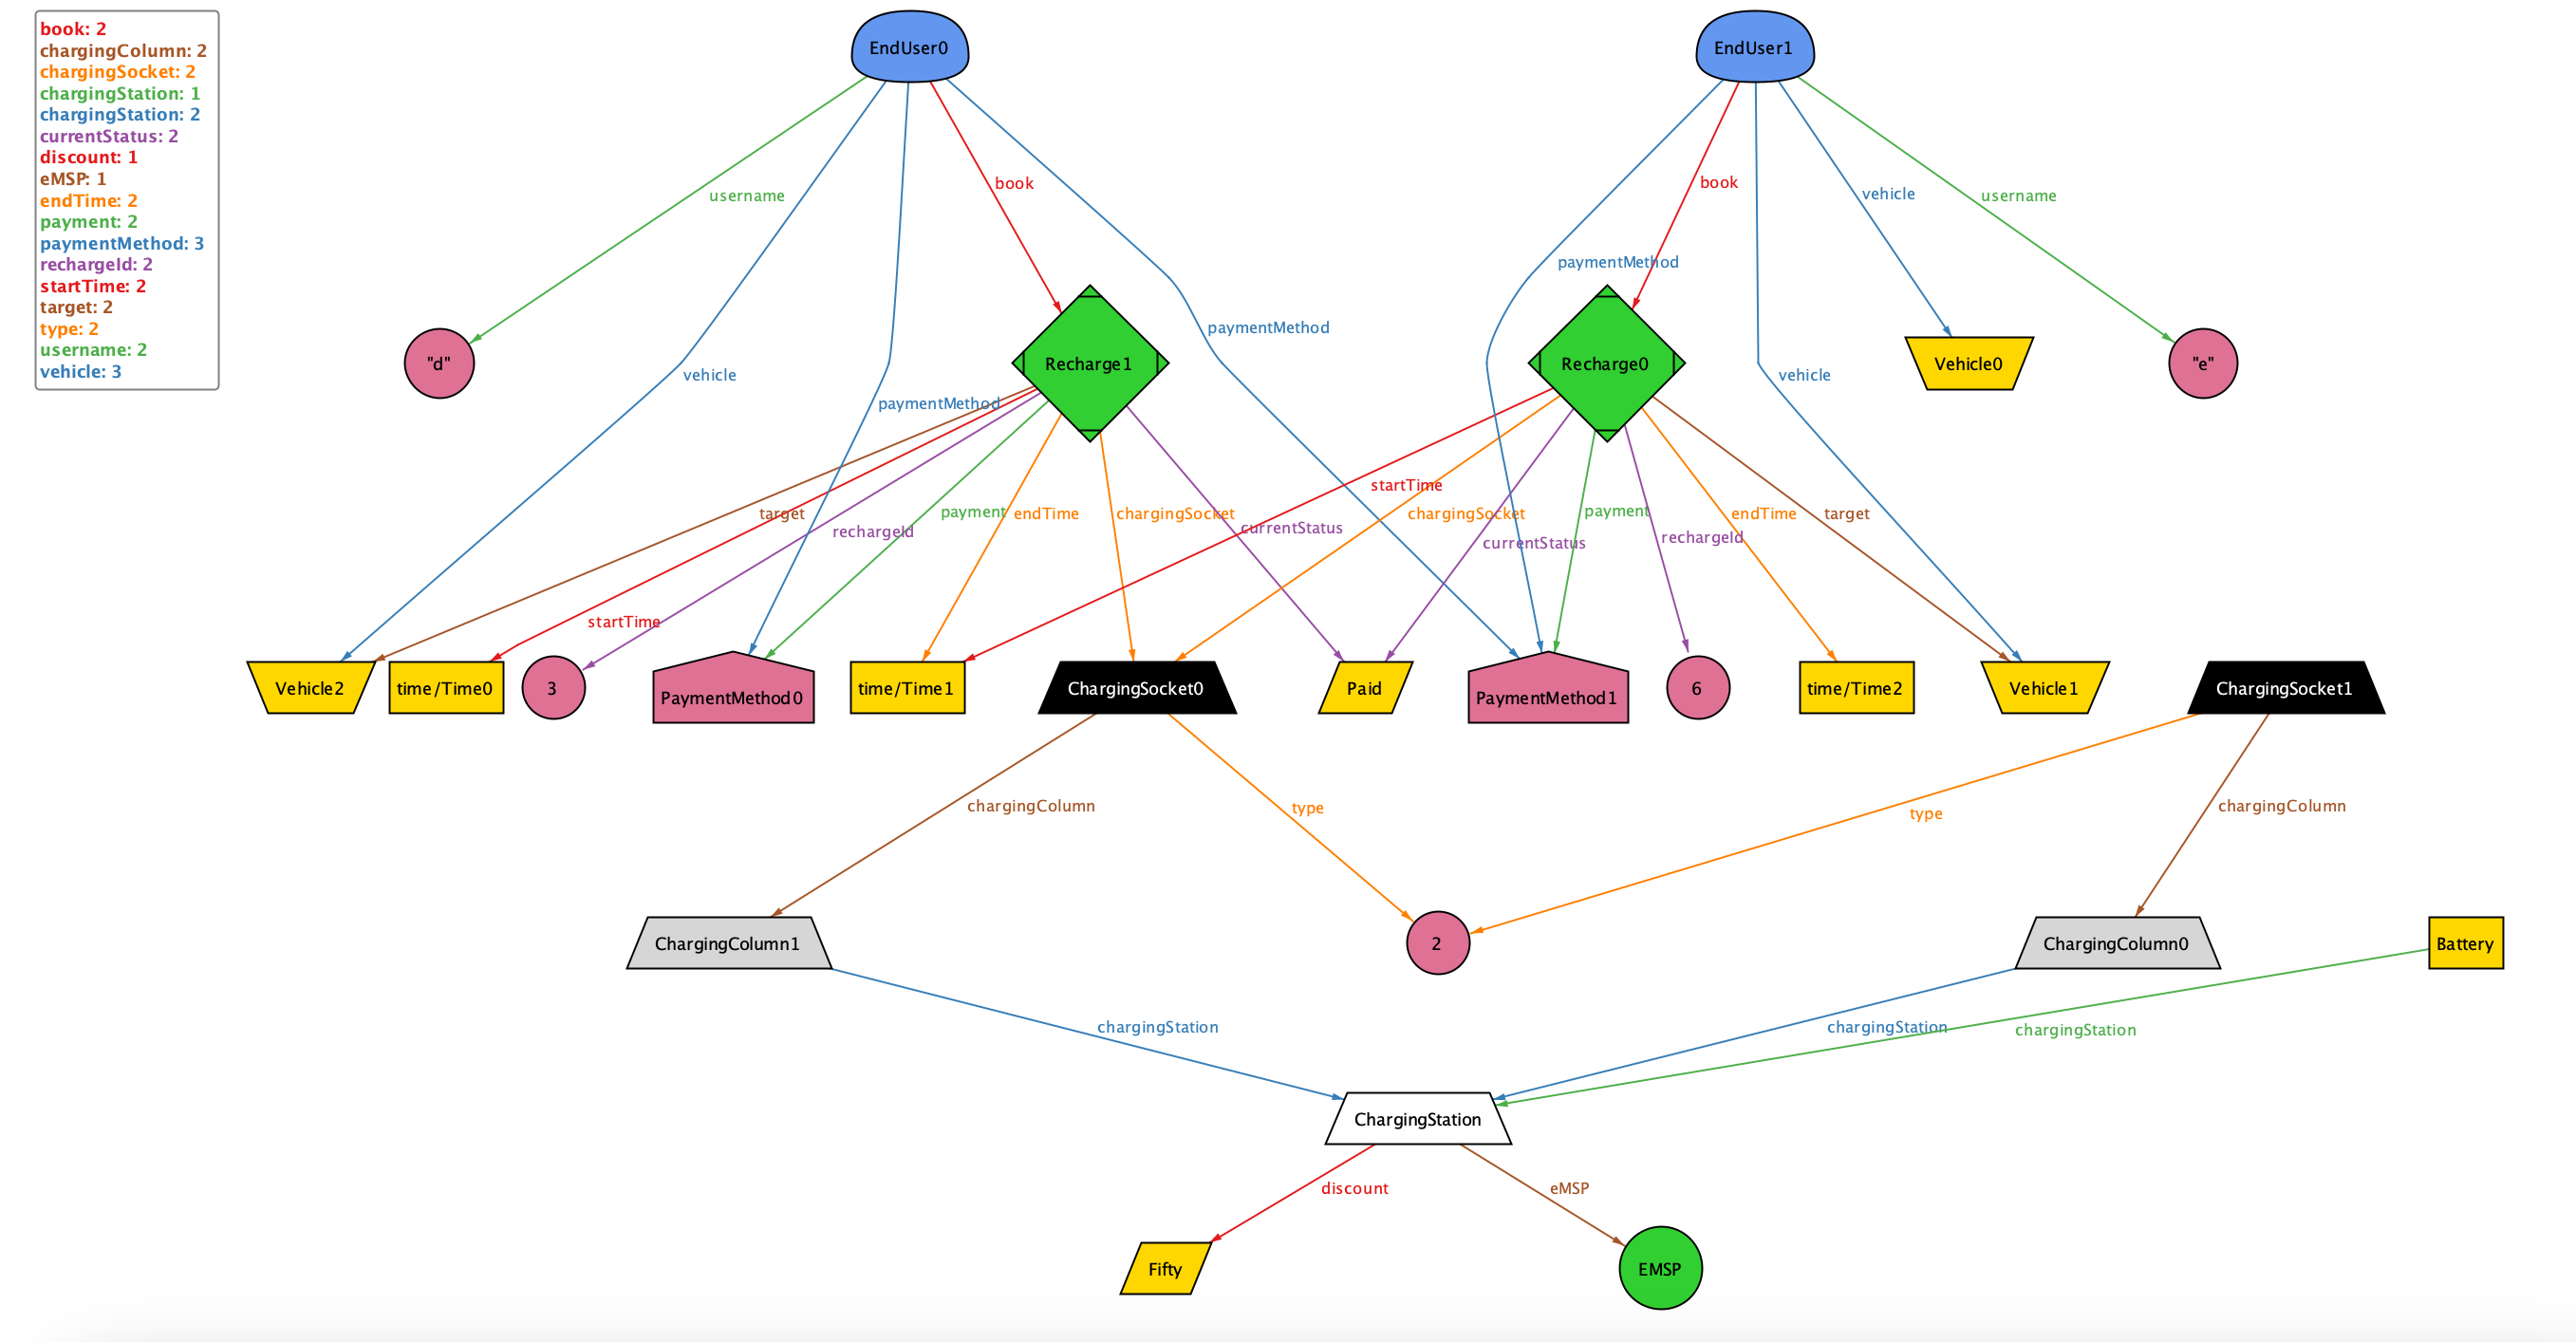
\includegraphics[angle=0, scale=0.55]{world1}
\caption{Alloy World n.1}
\label{fig:world1}
\end{figure}
\end{landscape}

\begin{landscape}
\begin{figure}[hp]
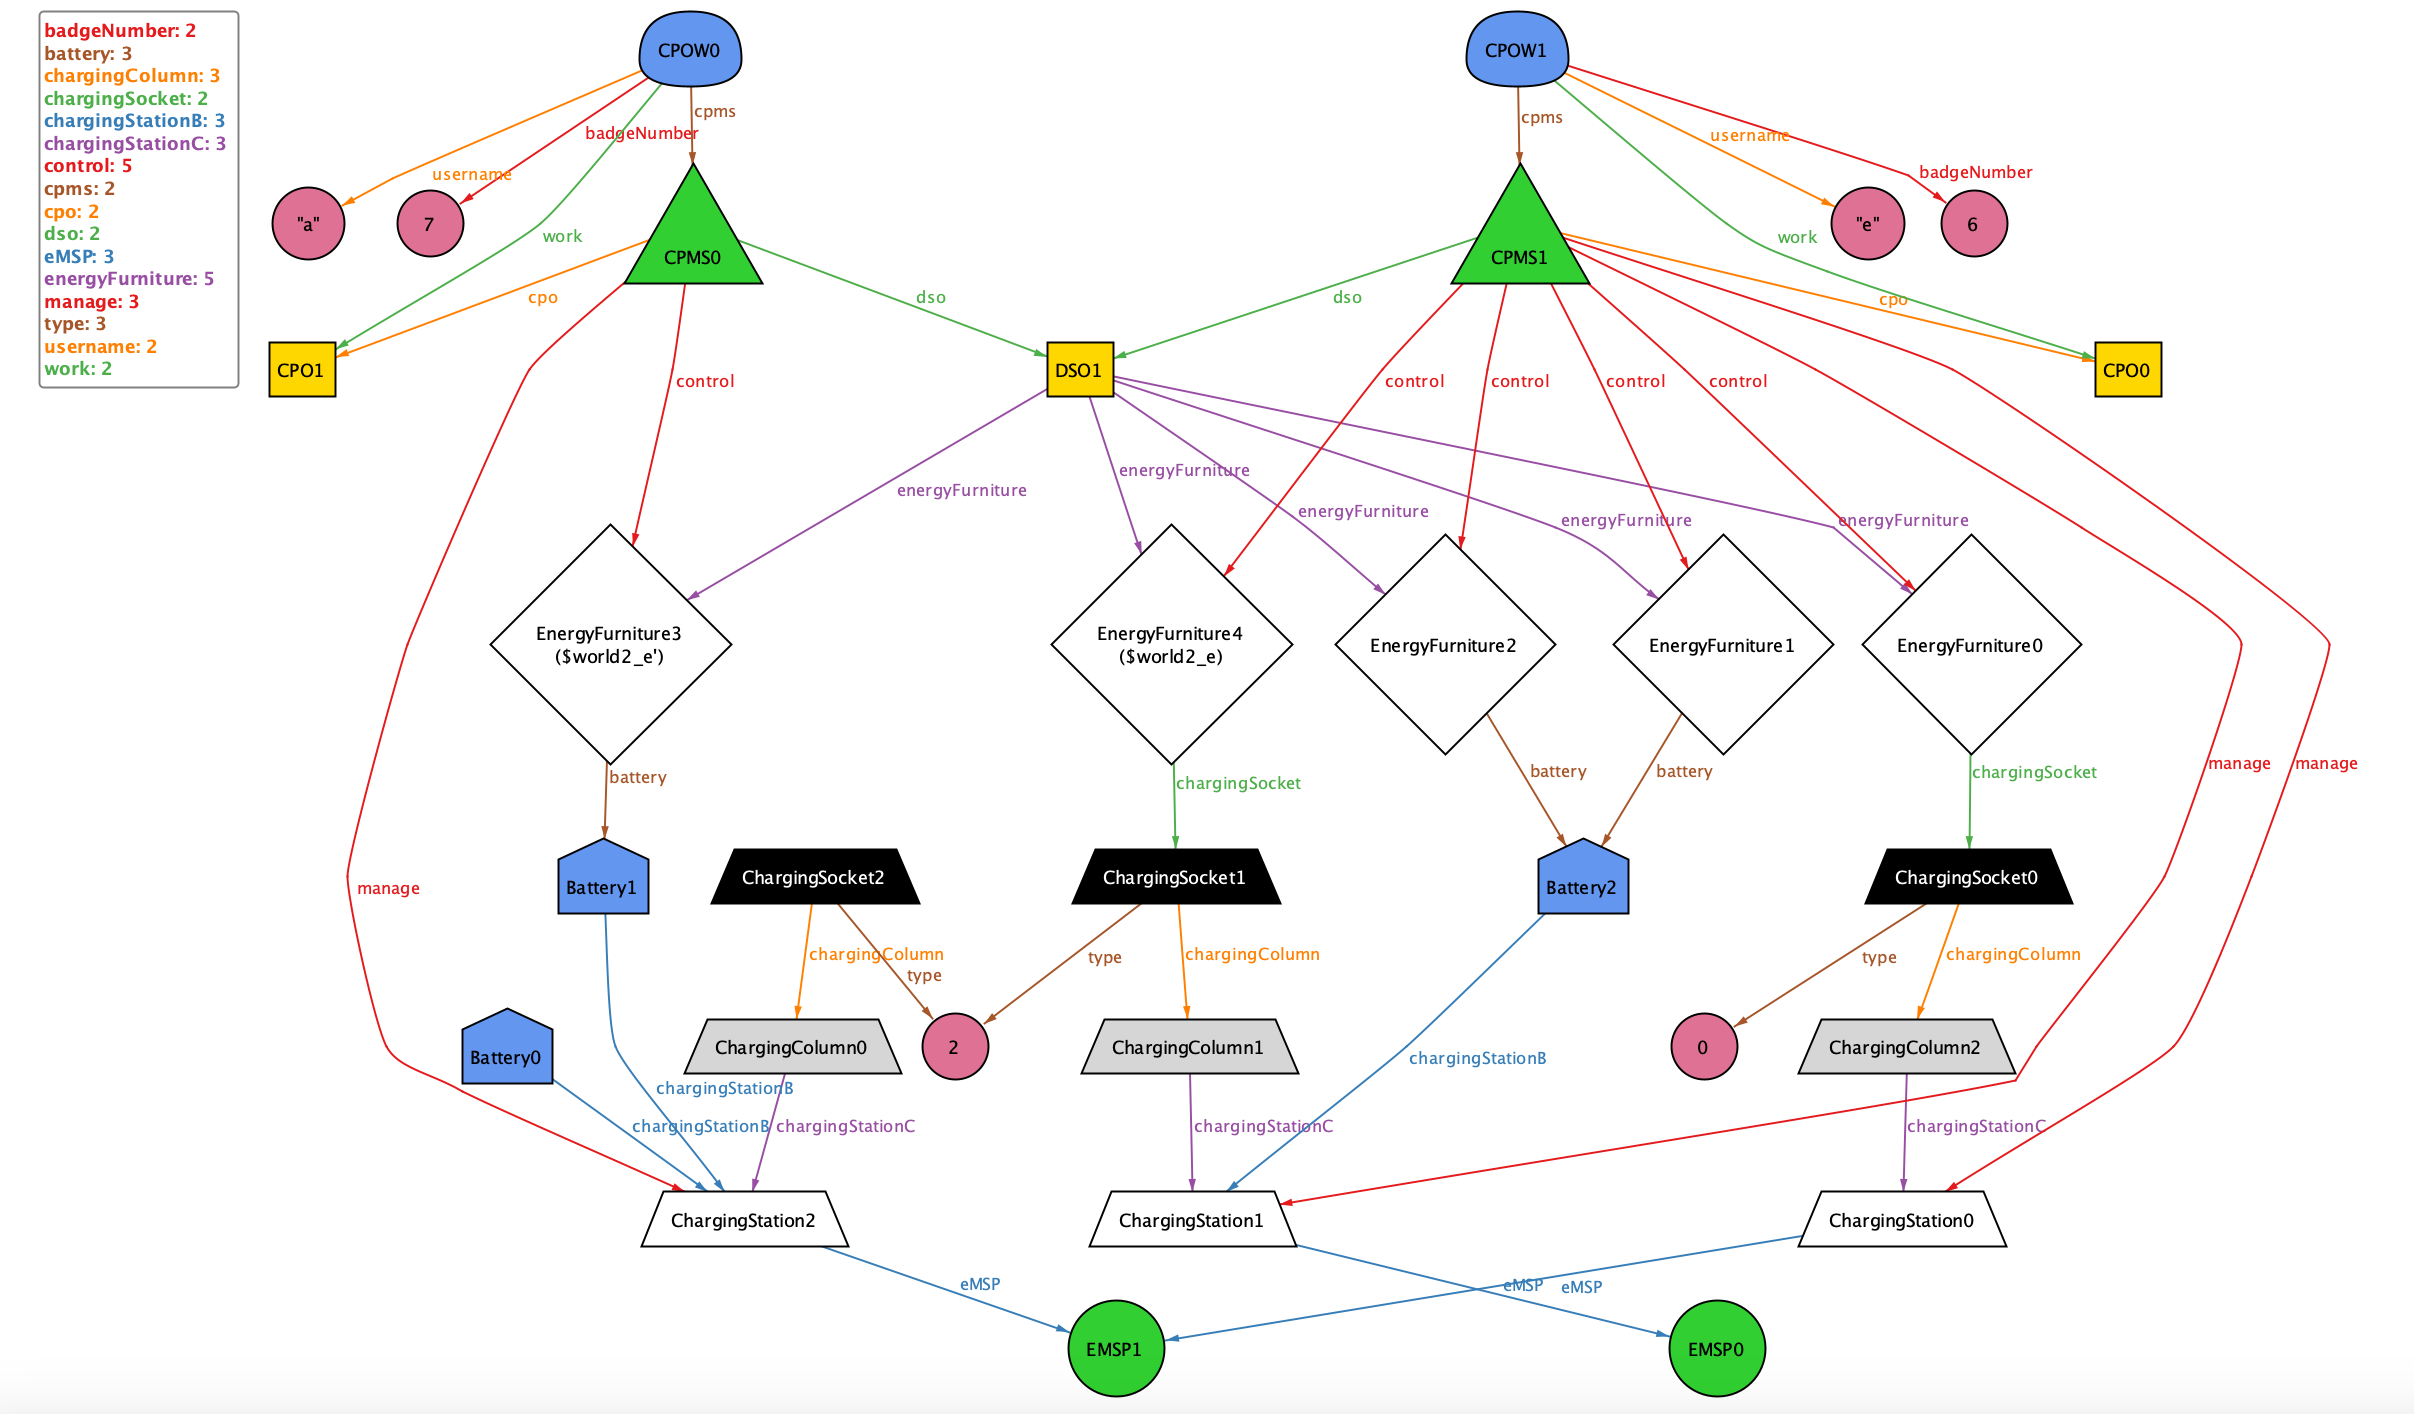
\includegraphics[angle=0, scale = 0.65]{world2}
\caption{Alloy World n.2}
\label{fig:world2}
\end{figure}
\end{landscape}

\begin{landscape}
\begin{figure}[hp]
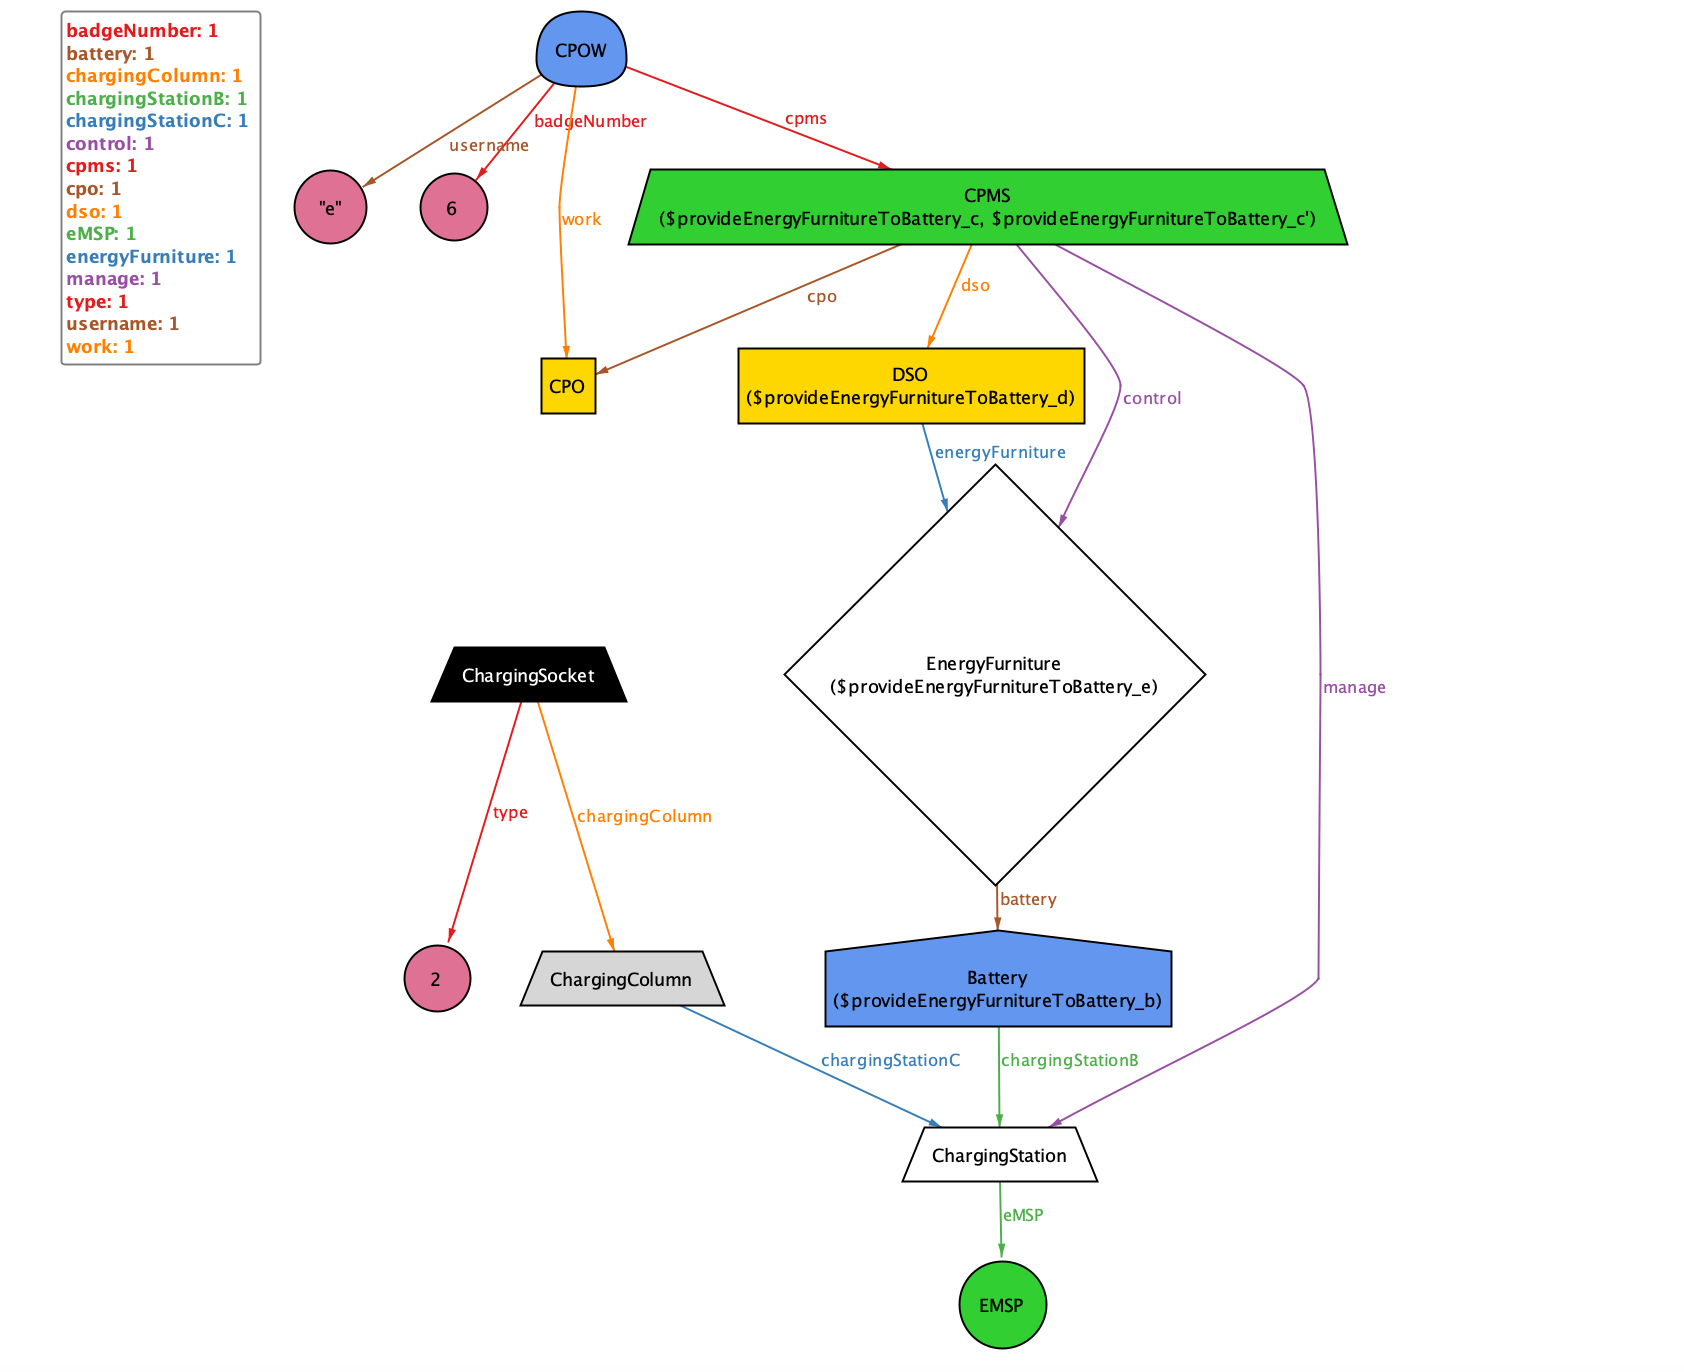
\includegraphics[angle=0, scale=0.6]{dynamicWorld}
\caption{Alloy predicate \textit{provideEnergyFurnitureToBattery}}
\label{fig:provideEnergy}
\end{figure}
\end{landscape}


\restoregeometry

\chapter{Effort spent}
\begin{table}[H]
\centering

Matteo Gionfriddo\\
\begin{tabular}{p{2cm}p{1.5cm}p{7cm}}
\toprule
\textit{Date} & \textit{Hour} & \textit{Section} \\ \midrule
09-11-2022 & 1.5 h* & Goals \\ \midrule
15-11-2022 & 1.5 h & World and Shared Phenomena and Table 1.1 \\ \midrule
19-11-2022 & 1 h & Use Cases\\ \midrule
22-11-2022 & 1 h & Use Cases \\ \midrule
27-11-2022 & 1 h & Use Cases \\ \midrule
29-11-2022 & 1 h & Use Cases \\ \midrule
30-11-2022 & 1 h* & Domain Assumptions \\ \midrule
04-12-2022 & 3 h* & Requirements \\ \midrule
07-12-2022 & 1.5 h & Use Cases and Table 3.2\\ \midrule
11-12-2022 & 2 h & UML Use Case Diagram\\  \midrule
13-12-2022 & 1.5 h & UML Use Case Diagram\\  \midrule
15-12-2022 & 1 h & Revision Use Cases\\ \midrule
17-12-2022 & 1.5 h & UML Sequence Diagram\\ \midrule
19-12-2022 & 2 h & UML Sequence Diagram\\ \midrule
20-12-2022 & 1.5 h & Table 3.1, Table 3.3 \\ \midrule
21-12-2022 & 2.5 h* & Final Revision \\ \midrule

\bottomrule
\end{tabular}
\caption[Matteo Gionfriddo's effort table]{}
\end{table}
\textit{* Group work}
\chapter{References}
\begin{itemize}
\item Specification Document: “Assignment RDD AY 2022-2023\_v3.pdf”
\item Alloy Reference Document Examples: “http://tmancini.di.uniroma1.it/teaching/courses/2007-2008/mfis/materiale/progetti/Pagliaro%20-%20Alloy.relazione.pdf"
\item IEEE Std 830-1993 - IEEE Guide to Software Requirements Specifications.
\item IEEE Std 830-1998 - IEEE Recommended Practice for Software Requirements Specifications.
\end{itemize}
\end{document}
